\documentclass[preprint,12pt]{elsarticle}
%DIF LATEXDIFF DIFFERENCE FILE
%DIF DEL backup_20260907/diff_old_flat.tex   Mon Sep  7 17:56:34 2026
%DIF ADD backup_20260907/diff_new_flat.tex   Mon Sep  7 21:50:05 2026
\usepackage{lmodern}
\usepackage{amsmath,amssymb}
\usepackage{graphicx}
\usepackage{booktabs}
\usepackage{multirow}
\usepackage{array}
\usepackage{xcolor}
\usepackage[section]{placeins}
\usepackage{float}
\usepackage{xr-hyper}
\usepackage{hyperref}
\externaldocument[S-]{supplementary}
\hypersetup{hidelinks,
%DIF 15c15
%DIF <   pdftitle={CanonFuse3D: Calibration-Free Dual-View 3D Pose Refinement via Human-Centric Fusion},
%DIF -------
  pdftitle={Calibration-Free Post-Estimation Fusion of Dual-View 3D Human Pose Streams: Robustness, Front-End Generalization, and Multi-View Extension}, %DIF > 
%DIF -------
  pdfauthor={Kaixu Chen, Qingyu Wang, Nan Luo, Chun Xie, Eiichi Naito, Toshitaka Kimura, Itaru Kitahara}}
\usepackage{lineno}
\setlength{\emergencystretch}{2em}
\journal{Image and Vision Computing}

% Upright prose, including class-generated headings and bibliography emphasis.
\AddToHook{begindocument/end}{%
  \renewcommand{\itshape}{\fontshape{n}\selectfont}%
  \renewcommand{\slshape}{\fontshape{n}\selectfont}%
}
\renewcommand{\textit}[1]{\textup{#1}}
\renewcommand{\emph}[1]{\textup{#1}}
%DIF PREAMBLE EXTENSION ADDED BY LATEXDIFF
%DIF UNDERLINE PREAMBLE %DIF PREAMBLE
\RequirePackage[normalem]{ulem} %DIF PREAMBLE
\RequirePackage{color}\definecolor{RED}{rgb}{1,0,0}\definecolor{BLUE}{rgb}{0,0,1} %DIF PREAMBLE
\providecommand{\DIFaddtex}[1]{{\protect\color{blue}\uwave{#1}}} %DIF PREAMBLE
\providecommand{\DIFdeltex}[1]{{\protect\color{red}\sout{#1}}} %DIF PREAMBLE
%DIF SAFE PREAMBLE %DIF PREAMBLE
\providecommand{\DIFaddbegin}{} %DIF PREAMBLE
\providecommand{\DIFaddend}{} %DIF PREAMBLE
\providecommand{\DIFdelbegin}{} %DIF PREAMBLE
\providecommand{\DIFdelend}{} %DIF PREAMBLE
\providecommand{\DIFmodbegin}{} %DIF PREAMBLE
\providecommand{\DIFmodend}{} %DIF PREAMBLE
%DIF FLOATSAFE PREAMBLE %DIF PREAMBLE
\providecommand{\DIFaddFL}[1]{\DIFadd{#1}} %DIF PREAMBLE
\providecommand{\DIFdelFL}[1]{\DIFdel{#1}} %DIF PREAMBLE
\providecommand{\DIFaddbeginFL}{} %DIF PREAMBLE
\providecommand{\DIFaddendFL}{} %DIF PREAMBLE
\providecommand{\DIFdelbeginFL}{} %DIF PREAMBLE
\providecommand{\DIFdelendFL}{} %DIF PREAMBLE
%DIF HYPERREF PREAMBLE %DIF PREAMBLE
\providecommand{\DIFadd}[1]{\texorpdfstring{\DIFaddtex{#1}}{#1}} %DIF PREAMBLE
\providecommand{\DIFdel}[1]{\texorpdfstring{\DIFdeltex{#1}}{}} %DIF PREAMBLE
%DIF AMSMATHULEM PREAMBLE %DIF PREAMBLE
\makeatletter %DIF PREAMBLE
\let\sout@orig\sout %DIF PREAMBLE
\renewcommand{\sout}[1]{\ifmmode\text{\sout@orig{\ensuremath{#1}}}\else\sout@orig{#1}\fi} %DIF PREAMBLE
\makeatother %DIF PREAMBLE
%DIF END PREAMBLE EXTENSION ADDED BY LATEXDIFF

\begin{document}

\begin{frontmatter}

\title{\DIFdelbegin \DIFdel{CanonFuse3D: }\DIFdelend Calibration-Free \DIFaddbegin \DIFadd{Post-Estimation Fusion of }\DIFaddend Dual-View 3D \DIFaddbegin \DIFadd{Human }\DIFaddend Pose \DIFdelbegin \DIFdel{Refinement via Human-Centric Fusion}\DIFdelend \DIFaddbegin \DIFadd{Streams: Robustness, Front-End Generalization, and Multi-View Extension}\DIFaddend \tnoteref{tnote:conference}}
\tnotetext[tnote:conference]{A preliminary version of this work has been accepted for publication at the 9th International Workshop on Multimedia Content Analysis in Sports (MMSports 2026). This article substantially extends that work.}

\author[ccs]{Kaixu Chen\corref{cor1}}
\ead{chenkaixusan@gmail.com}
\author[imiss]{Qingyu Wang}
\ead{wang.qingyu@image.iit.tsukuba.ac.jp}
\author[imiss]{Nan Luo}
\ead{nan.luo@image.iit.tsukuba.ac.jp}
\author[ccs]{Chun Xie}
\ead{xie.chun@image.iit.tsukuba.ac.jp}
\author[nict]{Eiichi Naito}
\ead{eiichi.naito@nict.go.jp}
\author[ntt]{Toshitaka Kimura}
\ead{toshitaka.kimura@ntt.com}
\author[ccs]{Itaru Kitahara}
\ead{kitahara.itaru@image.iit.tsukuba.ac.jp}

\cortext[cor1]{Corresponding author.}
\address[ccs]{Center for Computational Sciences, University of Tsukuba, Tsukuba, Ibaraki, Japan}
\address[imiss]{Intelligent and Mechanical Interaction Systems, University of Tsukuba, Tsukuba, Ibaraki, Japan}
\address[nict]{Advanced ICT Research Institute, National Institute of Information and Communications Technology, Osaka, Japan}
\address[ntt]{NTT Communication Science Laboratories, Tokyo, Japan}

\begin{abstract}
\DIFdelbegin \DIFdel{Recovering }\DIFdelend \DIFaddbegin \DIFadd{Multi-view capture can resolve the depth ambiguity, self-occlusion, and temporal jitter that limit monocular }\DIFaddend three-dimensional (3D) human \DIFdelbegin \DIFdel{motion from two distant viewpoints is challenging when the subject moves rapidly and camera calibration is unavailable}\DIFdelend \DIFaddbegin \DIFadd{pose estimation, but calibrated multi-view reconstruction is impractical when cameras follow a distant, fast-moving athlete or are installed temporarily. Two views are the smallest deployable multi-view configuration, and modern monocular estimators already deliver an independent 3D pose stream for each view}\DIFaddend . We present CanonFuse3D, a calibration-free post-estimation framework that \DIFdelbegin \DIFdel{refines }\DIFdelend \DIFaddbegin \DIFadd{fuses }\DIFaddend two approximately synchronized monocular 3D pose streams \DIFdelbegin \DIFdel{through human-centric fusion. The output consists of canonical joint coordinates relative to fixed, stream-specific body references; it does not represent a reconstructed world-space trajectory. Sequence-level pose alignment exposes }\DIFdelend \DIFaddbegin \DIFadd{directly in pose space. Human-centric canonicalization and sequence-level alignment expose }\DIFaddend cross-view agreement and disagreement\DIFdelbegin \DIFdel{, while joint features, bidirectional }\DIFdelend \DIFaddbegin \DIFadd{; a shared joint encoder, bidirectional cross-view }\DIFaddend attention, and temporal refinement \DIFdelbegin \DIFdel{support }\DIFdelend \DIFaddbegin \DIFadd{then drive }\DIFaddend joint-frame \DIFaddbegin \DIFadd{reliability-}\DIFaddend gated fusion with residual correction. \DIFdelbegin \DIFdel{We evaluate the framework using }\DIFdelend \DIFaddbegin \DIFadd{The framework is evaluated on }\DIFaddend three skiing datasets: \DIFdelbegin \DIFdel{two for quantitative assessment and one }\DIFdelend \DIFaddbegin \DIFadd{a synthetic Unity dataset with avatar ground truth, the real-world Ski-PTZ-Pose dataset, and author-collected dual-view recordings }\DIFaddend for qualitative deployment. \DIFdelbegin \DIFdel{Compared with }\DIFdelend \DIFaddbegin \DIFadd{Relative to }\DIFaddend canonical averaging, CanonFuse3D reduces \DIFaddbegin \DIFadd{the }\DIFaddend mean per-joint position error \DIFdelbegin \DIFdel{(MPJPE) on a shared body-joint subset }\DIFdelend by 44.5\% on Unity and 48.6\% on Ski-PTZ-Pose \DIFdelbegin \DIFdel{, where the latter measures agreement with a constructed canonical reference. Controlled input perturbations show gains across the tested view separationsand small timing errors, with failures under severe corruption. Experiments with }\DIFdelend \DIFaddbegin \DIFadd{and outperforms every non-learned fusion baseline in position, Procrustes-aligned, and acceleration error; a temporal convolutional baseline trained on the same data is competitive in position error, and a temporal smoother attains lower acceleration error at a much higher position error. The gains persist across camera separations, small timing and sampling-rate errors, and structured pose or image occlusion. The same architecture generalizes to }\DIFaddend alternative pose estimators \DIFdelbegin \DIFdel{show that transfer depends on the upstream error distribution and benefits from target-specific adaptation . Simple learned baselines achieve lower clean-input position or acceleration errors, so the findings support the usefulness and limits of human-centric dual-view refinement rather than universal accuracy superiority.
}%DIFDELCMD < 

%DIFDELCMD < %%%
\DIFdelend \DIFaddbegin \DIFadd{through lightweight adaptation and extends to additional cameras through pairwise composition.
}\DIFaddend \end{abstract}

\begin{keyword}
3D human pose estimation \sep dual-view fusion \sep \DIFaddbegin \DIFadd{post-estimation pose fusion }\sep \DIFaddend calibration-free refinement \sep human-centric representation \sep \DIFdelbegin \DIFdel{temporal refinement
}%DIFDELCMD < 

%DIFDELCMD < %%%
\DIFdelend \DIFaddbegin \DIFadd{front-end generalization
}\DIFaddend \end{keyword}

\end{frontmatter}

\linenumbers

\section{Introduction}

\DIFdelbegin \DIFdel{Recovering }\DIFdelend \DIFaddbegin \DIFadd{Three-dimensional (}\DIFaddend 3D\DIFdelbegin \DIFdel{human motion from two camera views is a computer-vision problem with practical value when a moving subject must be observed over a large area. At long capture distances, the body occupies fewer pixels, making limb localization difficult. Rapid movement introduces motion blur, changing body orientation , and short-lived occlusion. A second viewpoint can provide complementary evidence, but independently estimated monocular poses may still disagree in depth, limb configuration, and temporal continuity}\DIFdelend \DIFaddbegin \DIFadd{) human pose estimation from a single camera has advanced rapidly, from temporal lifting of 2D keypoints~\mbox{%DIFAUXCMD
\cite{pavllo2019videopose3d,zheng2021poseformer,li2022mhformer} }\hskip0pt%DIFAUXCMD
and pretrained motion representations~\mbox{%DIFAUXCMD
\cite{zhu2023motionbert} }\hskip0pt%DIFAUXCMD
to video-based body models~\mbox{%DIFAUXCMD
\cite{kocabas2020vibe} }\hskip0pt%DIFAUXCMD
and foundation-scale full-body estimators that operate on in-the-wild images~\mbox{%DIFAUXCMD
\cite{yang2026sam}}\hskip0pt%DIFAUXCMD
. These estimators make 3D motion analysis practical for sports, where joint trajectories support performance evaluation, skill assessment, and injury prevention. Their outputs nevertheless inherit the limitations of a single viewpoint: depth along the optical axis is ambiguous, limbs are frequently self-occluded, errors depend on the body orientation relative to the camera, and per-frame predictions jitter over time. Skiing exposes all of these weaknesses at once, because athletes move rapidly, are observed from a distance, and change orientation continuously~\mbox{%DIFAUXCMD
\cite{rhodin2018learning,chen2021sportscap}}\hskip0pt%DIFAUXCMD
}\DIFaddend .

\DIFdelbegin %DIFDELCMD < \begin{figure}[t]
%DIFDELCMD <   \centering
%DIFDELCMD <   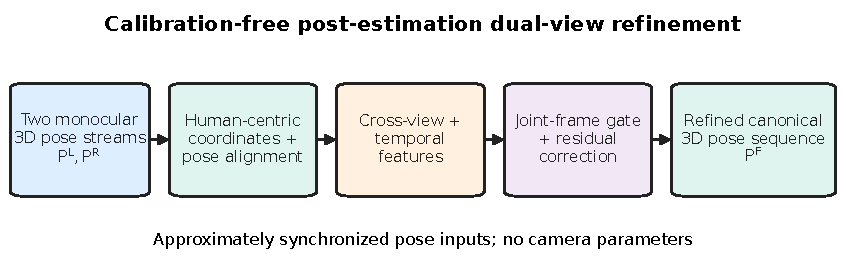
\includegraphics[width=0.98\linewidth]{figures/journal/study_overview.pdf}
%DIFDELCMD <   %%%
%DIFDELCMD < \caption{%
{%DIFAUXCMD
\DIFdelFL{System overview. Two monocular 3D pose streams are expressed in human-centric coordinates, aligned in pose space, and fused using cross-view and temporal features. CanonFuse3D produces a refined canonical pose sequence without camera parameters.}}
  %DIFAUXCMD
%DIFDELCMD < \label{fig:teaser}
%DIFDELCMD < \end{figure}
%DIFDELCMD < 

%DIFDELCMD < %%%
\DIFdelend \DIFaddbegin \DIFadd{Observing the athlete from complementary viewpoints is the established remedy. }\DIFaddend Calibrated multi-view \DIFdelbegin \DIFdel{reconstruction addresses these ambiguities through geometric constraints. Maintaining calibration is more difficult when cameras follow a distantsubject, change their orientation or zoom, or }\DIFdelend \DIFaddbegin \DIFadd{methods triangulate detections or fuse image features under known camera geometry and achieve high accuracy in laboratories and studios~\mbox{%DIFAUXCMD
\cite{nogueira2025survey,iskakov2019learnable,he2020epipolar,liao2024multiple,zhang2021adafuse}}\hskip0pt%DIFAUXCMD
. Field capture of a distant, fast-moving subject breaks their assumptions: cameras }\DIFaddend are installed temporarily \DIFdelbegin \DIFdel{in a large capture area. Existing monocular estimators also make independently predicted 3D pose streams readily available.
These conditions motivate a post-estimation question: how can two such streams be combined to improve pose quality when camera parameters are unavailable?
}%DIFDELCMD < 

%DIFDELCMD < %%%
\DIFdel{We address }\DIFdelend \DIFaddbegin \DIFadd{on a slope, pan and zoom to follow the athlete, and cannot be recalibrated before every session. Weakly calibrated and }\DIFaddend calibration-free \DIFdelbegin \DIFdel{post-estimation }\DIFdelend \DIFaddbegin \DIFadd{multi-view methods relax the camera requirements~\mbox{%DIFAUXCMD
\cite{usman2022metapose,gordon2022flex}}\hskip0pt%DIFAUXCMD
, but they still reconstruct the pose jointly from images or 2D detections and therefore replace, rather than build on, the monocular estimators that practitioners already run.
}

\DIFadd{These observations motivate a }\DIFaddend dual-view\DIFaddbegin \DIFadd{, post-estimation formulation. Two cameras form the smallest multi-view configuration: they are the cheapest to deploy and synchronize in the field, they already provide a second line of sight against depth ambiguity and self-occlusion, and, as we show later, they capture most of the accuracy available from larger camera groups at a fraction of the fusion cost. Because each view is processed by an off-the-shelf monocular estimator, the available data are two independently estimated }\DIFaddend 3D pose \DIFdelbegin \DIFdel{refinement. Calibration-free means that the refinement model receives no }\DIFdelend \DIFaddbegin \DIFadd{sequences rather than calibrated image observations. The problem addressed in this article is therefore to fuse two such streams into a more accurate and temporally stable pose sequence without }\DIFaddend camera intrinsics, extrinsics, \DIFaddbegin \DIFadd{or }\DIFaddend epipolar geometry, \DIFdelbegin \DIFdel{or triangulated image observations during }\DIFdelend \DIFaddbegin \DIFadd{at }\DIFaddend training or inference \DIFdelbegin \DIFdel{. Its inputs are two approximately synchronized 3D pose sequences. Human-centric coordinates reduce their global position and orientation discrepancy using body landmarks , and sequence-level similarity alignment provides an aligned opposite-view pose for each stream. The resulting representation describes motion relative to fixed body references and does not recover a shared world coordinate system. }\DIFdelend \DIFaddbegin \DIFadd{time.
}\DIFaddend 

\DIFdelbegin \DIFdel{The proposed CanonFuse3D framework combines each }\DIFdelend \DIFaddbegin \DIFadd{Figure~\ref{fig:teaser} summarizes the proposed CanonFuse3D framework. Both streams are first expressed in human-centric coordinates defined by body landmarks and aligned to each other by a sequence-level similarity transform, which exposes where the two estimates agree and where they conflict. For every joint and frame, the framework combines the }\DIFaddend view's \DIFaddbegin \DIFadd{own }\DIFaddend pose, the aligned opposite-view pose, \DIFdelbegin \DIFdel{cross-view disagreement}\DIFdelend \DIFaddbegin \DIFadd{their difference}\DIFaddend , and motion cues\DIFdelbegin \DIFdel{. Bidirectional }\DIFdelend \DIFaddbegin \DIFadd{; a shared joint encoder, bidirectional }\DIFaddend cross-view attention\DIFdelbegin \DIFdel{exchanges joint information, and temporal refinement models local motion continuity. A }\DIFdelend \DIFaddbegin \DIFadd{, and short-range temporal refinement then produce a }\DIFaddend joint-frame \DIFdelbegin \DIFdel{gate then weights }\DIFdelend \DIFaddbegin \DIFadd{reliability gate that weights the two }\DIFaddend view-specific pose candidates, together with a learned residual correction. \DIFdelbegin \DIFdel{This design uses complementary pose evidence after monocular estimation while keeping the upstream estimator }\DIFdelend \DIFaddbegin \DIFadd{The upstream estimator remains }\DIFaddend separate from the fusion model\DIFdelbegin \DIFdel{.
}\DIFdelend \DIFaddbegin \DIFadd{, so the framework can be placed behind any monocular 3D pose estimator that provides the common joint set.
}\DIFaddend 

\DIFdelbegin \DIFdel{Skiing provides a demanding application of distant capture and rapid human motion.
We use }\DIFdelend \DIFaddbegin \begin{figure}[t]
  \centering
  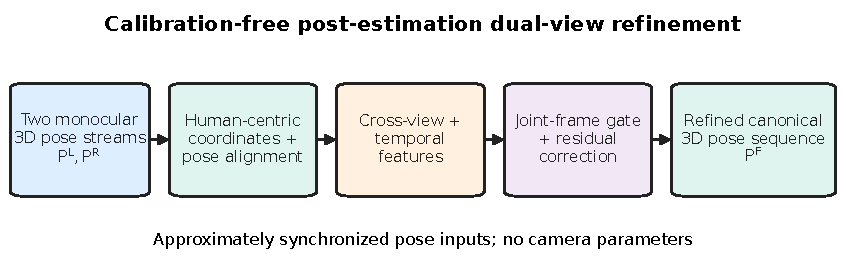
\includegraphics[width=0.98\linewidth]{figures/journal/study_overview.pdf}
  \caption{\DIFaddFL{System overview. Two monocular 3D pose streams are expressed in human-centric coordinates, aligned in pose space, and fused using cross-view and temporal features. CanonFuse3D produces a refined canonical pose sequence without camera parameters.}}
  \label{fig:teaser}
\end{figure}

\DIFadd{We evaluate the framework on }\DIFaddend three skiing datasets: \DIFdelbegin \DIFdel{Unity synthetic data and }\DIFdelend \DIFaddbegin \DIFadd{a synthetic Unity dataset with avatar ground truth, the }\DIFaddend public Ski-PTZ-Pose \DIFdelbegin \DIFdel{data for quantitative evaluation}\DIFdelend \DIFaddbegin \DIFadd{dataset with a constructed canonical reference}\DIFaddend , and author-collected indoor and outdoor recordings \DIFaddbegin \DIFadd{used }\DIFaddend for qualitative deployment. \DIFdelbegin \DIFdel{Unity provides recorded avatar skeletons; Ski-PTZ-Pose is evaluated against a constructed canonical reference derived from its annotations. Controlled }\DIFdelend \DIFaddbegin \DIFadd{Beyond clean-input accuracy, controlled }\DIFaddend studies examine how the same \DIFdelbegin \DIFdel{refinement framework behaves when capture conditions or upstream pose estimates change}\DIFdelend \DIFaddbegin \DIFadd{model behaves when the camera separation, timing, or sampling rate changes, when pose evidence or image regions are missing, when the upstream estimator is replaced, and when more than two cameras are available}\DIFaddend .

The main contributions are:
\begin{itemize}
    \item A human-centric framework for calibration-free post-estimation dual-view 3D pose \DIFdelbegin \DIFdel{refinement, motivated by distant capture of rapidly moving subjects}\DIFdelend \DIFaddbegin \DIFadd{fusion, combining landmark canonicalization, sequence-level alignment, cross-view attention, temporal refinement, and reliability-gated residual fusion}\DIFaddend .
    \item Quantitative evaluation on two skiing datasets with explicit reference regimes \DIFdelbegin \DIFdel{, complemented by a third dataset of }\DIFdelend \DIFaddbegin \DIFadd{against non-learned, learned, and calibrated fusion references, on which CanonFuse3D outperforms every non-learned baseline in position, Procrustes-aligned, and acceleration error, complemented by }\DIFaddend real-world deployment \DIFdelbegin \DIFdel{videos}\DIFdelend \DIFaddbegin \DIFadd{examples}\DIFaddend .
    \item \DIFdelbegin \DIFdel{An assessment of refinement under viewpoint and timing changes, pose and image corruption, alternative pose estimators, and additional input views, identifying both useful conditions and }\DIFdelend \DIFaddbegin \DIFadd{A systematic robustness analysis covering camera separation, timing and sampling-rate errors, and both pose-level and image-level occlusion, which identifies the useful operating range and its }\DIFaddend failure cases.
\end{itemize}

\section{Related Work}
\label{sec:related_work}

\subsection{Monocular \DIFdelbegin \DIFdel{and Sports }\DIFdelend 3D Human Pose Estimation}
Monocular 3D human pose estimation has progressed from temporal lifting models to transformer-based architectures and large-scale motion representation learning. VideoPose3D uses dilated temporal convolutions to lift 2D keypoint sequences into 3D poses~\cite{pavllo2019videopose3d}. PoseFormer models spatial joint relations and temporal correlations with transformers~\cite{zheng2021poseformer}. MHFormer represents multiple plausible pose hypotheses before synthesizing a final estimate~\cite{li2022mhformer}. MotionBERT pretrains a motion encoder on heterogeneous data for transfer to several human-centric tasks~\cite{zhu2023motionbert}. Recent full-body systems broaden the available front ends: SAM 3D Body estimates body, hand, and foot pose and shape from a single image and emphasizes generalization to diverse in-the-wild conditions~\cite{yang2026sam}, while VIBE uses a sequence-level adversarial motion prior to obtain kinematically plausible pose and shape estimates from video~\cite{kocabas2020vibe}. These methods improve the quality of an individual monocular stream, but they do not use a second synchronized stream to correct view-specific errors.

\DIFdelbegin \DIFdel{Sports footage makes }\DIFdelend \DIFaddbegin \DIFadd{In sports applications, }\DIFaddend the monocular problem \DIFdelbegin \DIFdel{especially difficult because professional }\DIFdelend \DIFaddbegin \DIFadd{is harder because athletic }\DIFaddend movements are rapid, atypical of common training corpora, and frequently self-occluded. \DIFaddbegin \DIFadd{Closest to our setting, }\DIFaddend Rhodin et al. introduced \DIFdelbegin \DIFdel{a skiing dataset with }\DIFdelend \DIFaddbegin \DIFadd{the Ski-Pose PTZ-Camera dataset of alpine skiers observed by }\DIFaddend rotating cameras and \DIFdelbegin \DIFdel{expert motion and }\DIFdelend used multi-view consistency \DIFdelbegin \DIFdel{mainly }\DIFdelend as supervision for a \DIFdelbegin \DIFdel{model that performs monocular inference~\mbox{%DIFAUXCMD
\cite{rhodin2018learning}}\hskip0pt%DIFAUXCMD
. SportsCap likewise }\DIFdelend \DIFaddbegin \DIFadd{monocular model~\mbox{%DIFAUXCMD
\cite{rhodin2018learning}}\hskip0pt%DIFAUXCMD
, and SportsCap }\DIFaddend targets monocular sports videos \DIFdelbegin \DIFdel{, using semantic and temporally structured }\DIFdelend \DIFaddbegin \DIFadd{with }\DIFaddend sub-motion priors\DIFdelbegin \DIFdel{to handle complex non-daily movements and severe self-occlusion}\DIFdelend ~\cite{chen2021sportscap}. \DIFdelbegin \DIFdel{These studies demonstrate the value of sports-specific data and motion priors. Their inference setting nevertheless remains monocular }\DIFdelend \DIFaddbegin \DIFadd{Both remain monocular at inference}\DIFaddend ; complementary 3D predictions from simultaneously available viewpoints are not fused after estimation.

\subsection{Multi-view 3D Pose Estimation}
A recent survey of markerless multi-view 3D human pose estimation emphasizes the benefits of complementary viewpoints while identifying occlusion, camera variation, limited supervision, temporal consistency, view selection, and the accuracy--complexity trade-off as continuing concerns~\cite{nogueira2025survey}. Classical and learned multi-view pipelines usually recover a single 3D pose inside the estimator. Learnable Triangulation combines per-view evidence through differentiable algebraic or volumetric triangulation~\cite{iskakov2019learnable}. Epipolar Transformers transfer image features along epipolar lines in a synchronized, calibrated setting~\cite{he2020epipolar}, and MVGFormer alternates appearance modules with learning-free geometric modules that triangulate refined 2D poses~\cite{liao2024multiple}. AdaFuse addresses unreliable or occluded views by estimating point correspondences between heatmaps and learning camera-specific fusion weights so that poor features do not corrupt stronger views~\cite{zhang2021adafuse}. Although these strategies use different fusion mechanisms, they operate on images, feature maps, heatmaps, or calibrated 2D observations as part of multi-view reconstruction rather than on independently produced 3D pose streams.

Other work relaxes calibration or supervision. MetaPose estimates 3D pose from multiple cameras with unknown calibration, models uncertainty in the input 2D keypoints, and requires only 2D keypoint data for training~\cite{usman2022metapose}. FLEX removes the need for extrinsic parameters by predicting view-invariant skeletal rotations and bone lengths from multiple video streams and fusing their learned features into one temporally coherent motion~\cite{gordon2022flex}. These methods substantially reduce camera requirements, but they still couple cross-view fusion to the multi-view reconstruction network. The setting studied here is complementary: the upstream estimators have already produced two monocular 3D sequences, and the refinement stage receives neither images nor 2D detections, camera parameters, or epipolar geometry.

Takahashi et al.~\cite{takahashi2018human} \DIFdelbegin \DIFdel{address the additional problem of temporal synchronization. Their method uses }\DIFdelend \DIFaddbegin \DIFadd{additionally recover temporal synchronization: using }\DIFaddend detected 2D \DIFdelbegin \DIFdel{human }\DIFdelend joints as correspondences\DIFdelbegin \DIFdel{and estimates }\DIFdelend \DIFaddbegin \DIFadd{, they jointly estimate }\DIFaddend camera extrinsics, inter-camera time offsets, and 3D joint positions \DIFdelbegin \DIFdel{through optimization with relaxed reprojection errors and human-body constraints. It therefore tackles }\DIFdelend \DIFaddbegin \DIFadd{from }\DIFaddend unsynchronized, uncalibrated \DIFdelbegin \DIFdel{reconstruction directly. CanonFuse3D instead receives two already-estimated 3D streams and learns a pose-space correction without recovering camera parameters; it still requires approximately corresponding times. This narrower input setting does not subsume the synchronization capability of Takahashi et al. The temporal perturbation experiments and auxiliary synchronization diagnostic below characterize }\DIFdelend \DIFaddbegin \DIFadd{cameras. Synchronization is therefore recoverable from human motion itself. In this work the two input streams are assumed to be approximately synchronized, and }\DIFaddend the remaining timing \DIFdelbegin \DIFdel{requirement, rather than establish equivalent reconstruction capability or a quantitative comparison with that method}\DIFdelend \DIFaddbegin \DIFadd{tolerance is characterized experimentally}\DIFaddend .

\subsection{Pose-Space Refinement, Reliability, and Generalization}
Post-estimation refinement provides another way to improve predictions without replacing the upstream estimator. STRIDE is a model-agnostic test-time training method that fits a motion prior to each video and refines noisy initial 3D estimates into temporally coherent poses under occlusion~\cite{lal2025stride}. Its objective is single-video temporal refinement rather than the reconciliation of synchronized viewpoints. Reliability weighting also appears within multi-view estimators: Learnable Triangulation predicts confidence weights for algebraic triangulation, and AdaFuse estimates adaptive weights for camera-view features~\cite{iskakov2019learnable,zhang2021adafuse}. In contrast, the reliability gate in this study acts after monocular 3D estimation and selects between aligned 3D pose candidates at the joint--frame level. The distinction is important because upstream confidence, image-feature quality, and residual pose-space reliability are not interchangeable signals.

Robust deployment also depends on how an estimator responds to a changed pose or camera distribution. PoseAug learns differentiable changes to posture, body size, viewpoint, and position to diversify paired 2D--3D training poses and improve cross-dataset generalization~\cite{gong2021poseaug}. AdaptPose instead generates target-like 3D motions and camera orientations from source poses and uses target-domain 2D poses without requiring target 3D labels or camera information~\cite{gholami2022adaptpose}. Both approaches adapt the training distribution of a 3D pose estimator. Our experiments address a different transfer boundary: they hold the pose-space fusion architecture fixed, replace the upstream monocular estimator, and then compare frozen transfer with target-specific adaptation of the refinement model.

These studies leave a complementary problem: fusing independently estimated 3D pose streams after monocular inference. CanonFuse3D addresses this problem through human-centric pose alignment, cross-view temporal reasoning, and joint-frame gating. The supporting experiments examine the conditions under which this refinement remains useful.

\section{Proposed Method}
\label{sec:method}

\subsection{Overview}
\label{subsec:method_overview}

CanonFuse3D takes independently estimated pose sequences \(P^L,P^R\in\mathbb{R}^{T\times J\times3}\) from two approximately synchronized views, where \(T\) is the number of frames and \(J\) the number of joints. It predicts a refined canonical pose sequence \(P^F\) of the same shape without camera parameters. Figure~\ref{fig:feature_construction} shows the \DIFdelbegin \DIFdel{five stages: }\DIFdelend \DIFaddbegin \DIFadd{complete pipeline. Stages 1--3 place both streams in }\DIFaddend human-centric \DIFdelbegin \DIFdel{canonicalization, bidirectional pose alignment, geometric-motion feature encoding, cross-view and temporal refinement, and gated pose fusion}\DIFdelend \DIFaddbegin \DIFadd{coordinates and align them to each other in pose space; stage 4 assembles, for every joint and frame, the five three-dimensional cues that describe the view's own estimate, the aligned opposite estimate, their disagreement, local motion, and the alignment rotation; stages 5--8 encode these cues, exchange information across views and over time, and fuse the two view-specific pose candidates through a reliability gate and a residual correction}\DIFaddend .

\DIFaddbegin \begin{figure}[!t]
  \centering
  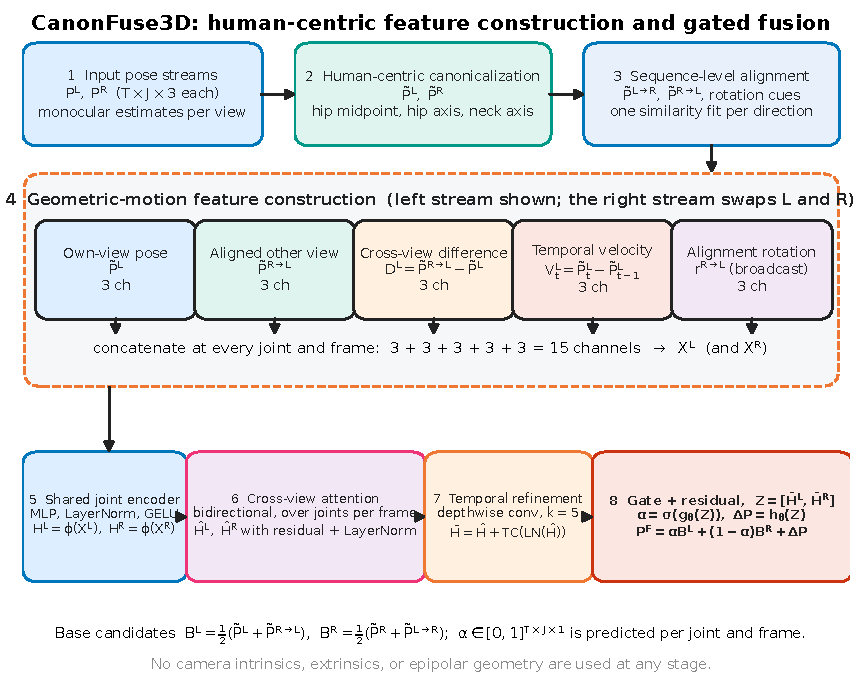
\includegraphics[width=0.98\linewidth]{figures/journal/method_pipeline.pdf}
  \caption{\DIFaddFL{CanonFuse3D pipeline and feature construction. Stages 1--3 canonicalize and align the two pose streams; stage 4 concatenates five three-dimensional cues (own-view pose, aligned opposite-view pose, their difference, temporal velocity, and alignment rotation) into a 15-channel feature at every joint and frame; stages 5--8 encode the features, apply bidirectional cross-view attention and temporal refinement, and fuse the two base candidates \(B^L\) and \(B^R\) through a joint-frame gate \(\alpha\) with a residual correction \(\Delta P\). The right stream uses the same construction with the view roles reversed.}}
  \label{fig:feature_construction}
\end{figure}

\DIFaddend \subsection{Human-Centric Landmark Canonicalization}
\label{subsec:canonicalization}

Independent monocular estimates can differ in global position and orientation. We express each stream relative to a fixed reference pose \(A\) using the hip midpoint, hip direction, and neck direction. Let \(h_L,h_R,n\) denote the left hip, right hip, and neck, and let \(\operatorname{nrm}(v)=v/(\|v\|_2+\epsilon)\). The origin and body axes are
\[
\begin{aligned}
c&=\tfrac12(A_{h_L}+A_{h_R}), &
e_x&=\operatorname{nrm}(A_{h_R}-A_{h_L}),\\
e_y&=\operatorname{nrm}(A_n-c), &
e_z&=\operatorname{nrm}(e_x\times e_y).
\end{aligned}
\]
An additional landmark-direction cue resolves the sign of \(e_z\). With the axis matrix \(R=[e_x,e_y,e_z]\), the transformed coordinates are
\[
\tilde{P}_{t,j}=(P_{t,j}-c)R.
\]
The left stream, right stream, and supervision reference use separate body references. Each origin and axis matrix remains fixed over the sequences to which it is applied; the representation is therefore not a per-frame root-relative pose. Skeleton scale is not normalized, and the constructed axes need not be orthogonal. In the evaluated protocol, the reference is shared within each batch. Its exact selection and landmark conventions are specified in Supplementary Section~\ref{S-sec:implementation_record}.

\subsection{Pose-Level Cross-View Alignment}
\label{subsec:pose_alignment}

Because the independently anchored streams can retain residual translation, orientation, and scale mismatch, we apply pose-level cross-view alignment in both directions. Specifically, the left pose sequence is aligned to the right pose sequence, and the right pose sequence is aligned to the left pose sequence:
\[
\tilde{P}^{L \rightarrow R} = \mathcal{A}(\tilde{P}^{L}, \tilde{P}^{R}),
\qquad
\tilde{P}^{R \rightarrow L} = \mathcal{A}(\tilde{P}^{R}, \tilde{P}^{L}),
\]
where \(\mathcal{A}(\cdot)\) denotes sequence-level pose alignment.

For each sample, let \(X,Y\in\mathbb{R}^{N\times3}\) contain the source and destination joint coordinates in row-vector form, with \(N=TJ\). We estimate one uniform scale \(s\), proper rotation \(Q\), and translation \(d\) for the whole sequence:
\[
(s^\star,Q^\star,d^\star)=
\underset{s\geq0,\;Q\in SO(3),\;d\in\mathbb{R}^{3}}{\arg\min}
\frac{1}{N}\left\|sXQ^\top+\mathbf{1}d^\top-Y\right\|_F^2.
\]
We solve this unweighted least-squares problem by singular value decomposition, excluding reflections. Each direction uses one transform for all frames and joints in the sequence. These auxiliary pose-space transforms do not estimate camera extrinsics; they are also distinct from the per-frame reference alignment used only for evaluation.

The model requires dense, finite pose tensors and receives no joint-validity mask. Missing detections are represented by zero-filled raw poses, and the controlled pose-corruption study replaces or perturbs selected raw entries before canonicalization. All transformed entries participate equally in alignment and training, including corrupted or zero-filled entries; missing joints are neither interpolated nor omitted. Detection-failure flags are used only for reporting, and supervision references remain uncorrupted. Supplementary Section~\ref{S-sec:controlled_details} gives the intervention rules.

We further compute cross-view residuals:
\[
D^{L} = \tilde{P}^{R \rightarrow L} - \tilde{P}^{L},
\qquad
D^{R} = \tilde{P}^{L \rightarrow R} - \tilde{P}^{R}.
\]
These residuals encode disagreement between the two pose streams and provide cues about view-specific errors.

\subsection{Geometric-Motion Feature Construction}
\label{subsec:feature_construction}

\DIFdelbegin %DIFDELCMD < \begin{figure}[t]
%DIFDELCMD <   \centering
%DIFDELCMD <   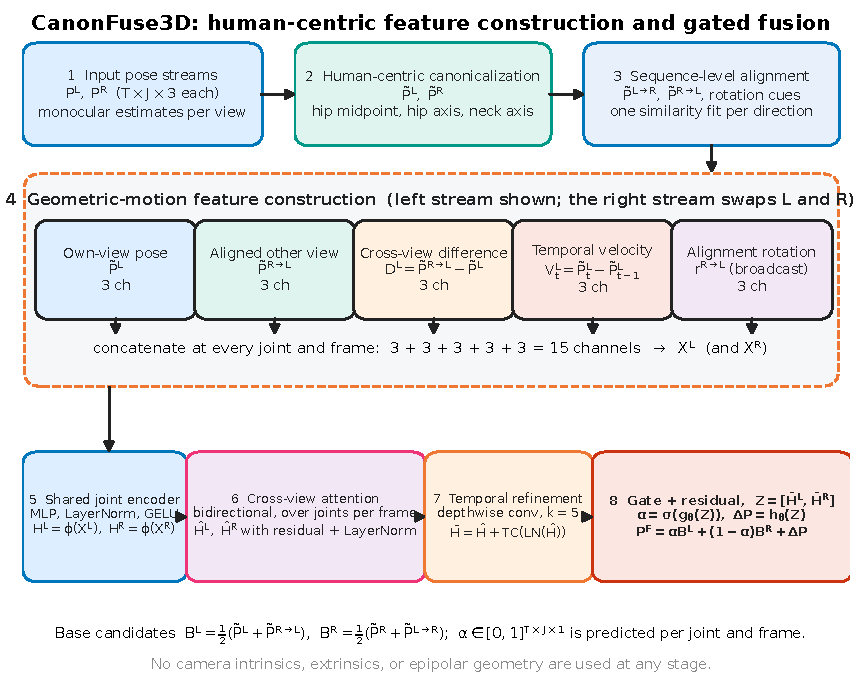
\includegraphics[width=0.98\linewidth]{figures/journal/method_pipeline.pdf}
%DIFDELCMD <   %%%
%DIFDELCMD < \caption{%
{%DIFAUXCMD
\DIFdelFL{CanonFuse3D architecture. Human-centric coordinates and sequence-level alignment provide geometric-motion features for cross-view attention and temporal refinement. A joint-frame gate and residual head produce the refined pose. The feature construction in stage 4 is detailed in Figure~\ref{fig:feature_details}.}}
  %DIFAUXCMD
%DIFDELCMD < \label{fig:feature_construction}
%DIFDELCMD < \end{figure}
%DIFDELCMD < 

%DIFDELCMD < %%%
\DIFdelend As shown in \DIFaddbegin \DIFadd{stage 4 of }\DIFaddend Figure~\ref{fig:feature_construction}, for each view \DIFdelbegin \DIFdel{, }\DIFdelend we construct joint-level geometric-motion features by concatenating pose, cross-view, and temporal cues. For the left-view stream, the feature is defined as
\[
X^{L}
=
\left[
\tilde{P}^{L},
\tilde{P}^{R \rightarrow L},
D^{L},
V^{L},
r^{R \rightarrow L}
\right],
\]
and for the right-view stream,
\[
X^{R}
=
\left[
\tilde{P}^{R},
\tilde{P}^{L \rightarrow R},
D^{R},
V^{R},
r^{L \rightarrow R}
\right].
\]
\DIFdelbegin %DIFDELCMD < 

%DIFDELCMD < %%%
\DIFdelend The velocity terms \DIFdelbegin \DIFdel{\(V^L,V^R\) describe frame-to-frame canonical pose changes, }\DIFdelend \DIFaddbegin \DIFadd{are first temporal differences of the canonical poses, \(V^{L}_{t}=\tilde{P}^{L}_{t}-\tilde{P}^{L}_{t-1}\) with \(V^{L}_{1}=0\), and likewise for \(V^{R}\). The terms \(r^{R \rightarrow L}\) }\DIFaddend and \DIFdelbegin \DIFdel{\(r^{R \rightarrow L},r^{L \rightarrow R}\) encode the corresponding alignment rotations. As shown in Figure~\ref{fig:feature_details}, the five }\DIFdelend \DIFaddbegin \DIFadd{\(r^{L \rightarrow R}\) are the rotation vectors of the corresponding sequence-level alignment rotations, broadcast to all joints and frames of the sequence. Each cue is }\DIFaddend three-dimensional\DIFdelbegin \DIFdel{cues are concatenated into }\DIFdelend \DIFaddbegin \DIFadd{, so every joint at every frame is described by }\DIFaddend a 15-dimensional feature \DIFdelbegin \DIFdel{for each joint and frame}\DIFdelend \DIFaddbegin \DIFadd{vector. The five cues give the network the view's own estimate, the opposite view expressed in the same pose space, the residual disagreement between them, local motion, and the global relation between the two streams; together they are the evidence from which the reliability of each candidate is inferred}\DIFaddend .

\DIFdelbegin %DIFDELCMD < \begin{figure}[t]
%DIFDELCMD < \centering
%DIFDELCMD < 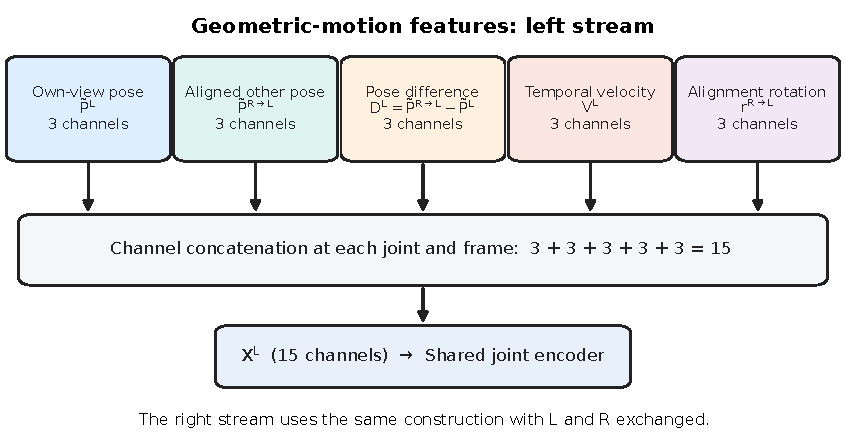
\includegraphics[width=0.98\linewidth]{figures/journal/feature_details.pdf}
%DIFDELCMD < %%%
%DIFDELCMD < \caption{%
{%DIFAUXCMD
\DIFdelFL{Geometric-motion feature construction for the left stream. Five three-dimensional cues are concatenated at each joint and frame: the own-view pose, aligned opposite-view pose, their difference, temporal velocity, and alignment rotation. The right stream uses the same construction with the view roles reversed.}}
%DIFAUXCMD
%DIFDELCMD < \label{fig:feature_details}
%DIFDELCMD < \end{figure}
%DIFDELCMD < 

%DIFDELCMD < %%%
\DIFdelend \subsection{Joint Feature Encoding}
\label{subsec:joint_feature_encoding}

The left and right geometric-motion features are passed through a shared joint-wise encoder:
\[
H^{L} = \phi(X^{L}),
\qquad
H^{R} = \phi(X^{R}),
\]
where \(\phi(\cdot)\) is a \DIFdelbegin \DIFdel{multilayer perceptron with layer }\DIFdelend \DIFaddbegin \DIFadd{two-layer multilayer perceptron, each layer followed by layer }\DIFaddend normalization and GELU activation. The encoder maps the 15-dimensional input feature into a \DIFaddbegin \DIFadd{128-dimensional }\DIFaddend hidden representation for each joint and frame.

Because the encoder is applied at the joint-feature level, it preserves the temporal and skeletal structure of the input sequence while producing a richer representation for subsequent cross-view interaction.

\subsection{Bidirectional Cross-View Attention}
\label{subsec:cross_view_attention}

To exchange complementary information between the two pose streams, we use bidirectional cross-view attention. For each frame, the left-view joint features attend to the right-view joint features, and the right-view joint features attend to the left-view joint features:
\[
\hat{H}^{L}
=
\DIFaddbegin \DIFadd{\mathrm{LN}\!}\left(\DIFadd{H^{L}+}\DIFaddend \mathrm{Attn}(Q=H^{L}, K=H^{R}, V=H^{R})\DIFaddbegin \right)\DIFaddend ,
\]
\[
\hat{H}^{R}
=
\DIFaddbegin \DIFadd{\mathrm{LN}\!}\left(\DIFadd{H^{R}+}\DIFaddend \mathrm{Attn}(Q=H^{R}, K=H^{L}, V=H^{L})\DIFaddbegin \right)\DIFaddend .
\]
\DIFdelbegin %DIFDELCMD < 

%DIFDELCMD < %%%
\DIFdelend The attention is \DIFdelbegin \DIFdel{applied over }\DIFdelend \DIFaddbegin \DIFadd{multi-head and is applied over the \(J\) }\DIFaddend joints within each frame\DIFaddbegin \DIFadd{, with separate parameters for the two directions}\DIFaddend . This allows the network to compare corresponding and related joint features across the two views. When a joint is unreliable in one view, the other view may provide complementary information. \DIFdelbegin \DIFdel{Residual connections }\DIFdelend \DIFaddbegin \DIFadd{The residual connection }\DIFaddend and layer normalization \DIFdelbegin \DIFdel{are used to }\DIFdelend stabilize the cross-view feature update.

\subsection{Temporal Refinement}
\label{subsec:temporal_refinement}

Frame-wise fusion alone may reduce spatial error but can still produce temporally unstable pose trajectories. To address this issue, we apply a temporal refinement module after cross-view attention.

The temporal refiner \DIFdelbegin \DIFdel{uses depthwise one-dimensional convolution along the time dimension. For each joint, the hidden feature }\DIFdelend \DIFaddbegin \DIFadd{operates on each joint's hidden feature trajectory. The }\DIFaddend sequence is normalized and passed through a \DIFdelbegin \DIFdel{temporal convolution block}\DIFdelend \DIFaddbegin \DIFadd{depthwise one-dimensional convolution of kernel size 5 along time, a GELU activation, dropout, and a pointwise convolution}\DIFaddend :
\[
\bar{H} = \hat{H} + \mathrm{TempConv}(\mathrm{LN}(\hat{H})).
\]
This residual formulation preserves the original cross-view representation while adding local temporal context. The temporal module is lightweight and targets short-range motion consistency, which is important for reducing jitter in sports pose sequences. \DIFaddbegin \DIFadd{The same module is applied to \(\hat{H}^{L}\) and \(\hat{H}^{R}\).
}\DIFaddend 

\subsection{Reliability-Gated Fusion and Residual Correction}
\label{subsec:reliability_fusion}

After cross-view attention and temporal refinement, the left and right hidden features are concatenated:
\[
Z = [\bar{H}^{L}, \bar{H}^{R}].
\]
A gate head predicts a joint-frame reliability gate:
\[
\alpha = \sigma(g_{\theta}(Z)),
\]
where \DIFaddbegin \DIFadd{\(g_{\theta}\) is a two-layer perceptron with GELU activation, \(\sigma\) is the logistic function, and }\DIFaddend \(\alpha \in [0,1]^{T \times J \times 1}\). The gate controls the relative contribution of the two view-specific pose candidates for each joint and frame.

The two streams have separate body references. The network combines their view-specific candidates through a learned pose-space mapping; this combination does not imply a shared physical coordinate frame.

We construct two base pose candidates:
\[
B^{L} = \frac{1}{2}(\tilde{P}^{L} + \tilde{P}^{R \rightarrow L}),
\DIFaddbegin \DIFadd{\qquad
B^{R} = \frac{1}{2}(}\tilde{P}\DIFadd{^{R} + }\tilde{P}\DIFadd{^{L \rightarrow R}).
}\DIFaddend \]
\DIFdelbegin \[
\DIFdel{B^{R} = \frac{1}{2}(\tilde{P}^{R} + \tilde{P}^{L \rightarrow R}).
}\]%DIFAUXCMD
\DIFdelend The reliability-gated base fusion is then computed as
\[
P^{base}
=
\alpha B^{L}
+
(1-\alpha)B^{R}.
\]

Finally, a residual head \DIFaddbegin \DIFadd{with the same two-layer structure }\DIFaddend predicts a pose correction:
\[
\Delta P = h_{\theta}(Z),
\]
and the final refined pose is
\[
P^{F} = P^{base} + \Delta P.
\]

The gate \(\alpha\) is interpreted as a learned reliability signal rather than a calibrated probabilistic uncertainty estimate. This distinction is important because the model is trained to improve fusion accuracy and temporal stability, not to produce calibrated uncertainty values.

\subsection{Training Objective}
\label{subsec:training_objective}

The model is trained with a supervised pose loss and \DIFaddbegin \DIFadd{four }\DIFaddend lightweight regularization terms:
\[
\mathcal{L}
=
\mathcal{L}_{sup}
+
\lambda_{view}\mathcal{L}_{view}
+
\lambda_{bal}\mathcal{L}_{bal}
+
\lambda_{ent}\mathcal{L}_{ent}
+
\lambda_{temp}\mathcal{L}_{temp}.
\]
The supervised term is \DIFdelbegin \DIFdel{\(\mathcal{L}_{sup}=\|P^F-\tilde{G}\|_1\), where }\DIFdelend \DIFaddbegin \DIFadd{the mean absolute error to the independently canonicalized reference }\DIFaddend \(\tilde{G}\)\DIFdelbegin \DIFdel{is the independently canonicalized supervision reference . The view reconstruction }\DIFdelend \DIFaddbegin \DIFadd{,
}\[
\DIFadd{\mathcal{L}_{sup}=\frac{1}{3TJ}\sum_{t,j}\|P^{F}_{t,j}-\tilde{G}_{t,j}\|_{1}.
}\]
\DIFadd{The view-reconstruction }\DIFaddend term preserves the discrepancy between the two \DIFdelbegin \DIFdel{independently }\DIFdelend canonicalized inputs. \DIFdelbegin \DIFdel{Let }\DIFdelend \DIFaddbegin \DIFadd{With }\DIFaddend \(\delta=\tilde{P}^{L}-\tilde{P}^{R}\)\DIFdelbegin \DIFdel{. The view-consistency objective reconstructs }\DIFdelend \DIFaddbegin \DIFadd{, the fused pose and gate reconstruct the two inputs as }\DIFaddend \(\hat{P}^{L}=P^{F}+(1-\alpha)\delta\) and \(\hat{P}^{R}=P^{F}-\alpha\delta\), and
\DIFdelbegin \DIFdel{averages their \(L_1\) errors to \(\tilde{P}^{L}\) and \(\tilde{P}^{R}\), respectively. }\DIFdelend \DIFaddbegin \[
\DIFadd{\mathcal{L}_{view}=\frac{1}{2}\left(\frac{1}{3TJ}\sum_{t,j}\|\hat{P}^{L}_{t,j}-\tilde{P}^{L}_{t,j}\|_{1}
+\frac{1}{3TJ}\sum_{t,j}\|\hat{P}^{R}_{t,j}-\tilde{P}^{R}_{t,j}\|_{1}\right).
}\]
\DIFaddend This term constrains the gate and fused estimate without treating the sequence-level similarity transforms as physical camera geometry. \DIFdelbegin \DIFdel{To }\DIFdelend \DIFaddbegin \DIFadd{Two gate penalties }\DIFaddend avoid degenerate fusion\DIFdelbegin \DIFdel{, \(\mathcal{L}_{bal}=|\mathrm{mean}(\alpha)-0.5|\) }\DIFdelend \DIFaddbegin \DIFadd{: the balance term \(\mathcal{L}_{bal}=|\bar{\alpha}-0.5|\), where \(\bar{\alpha}\) is the mean gate over all joints and frames, }\DIFaddend discourages collapse to a single view, \DIFdelbegin \DIFdel{while an entropy term
}\DIFdelend \DIFaddbegin \DIFadd{and the negative-entropy term
}\[
\DIFadd{\mathcal{L}_{ent}=\frac{1}{TJ}\sum_{t,j}\left[\alpha_{t,j}\log\alpha_{t,j}+(1-\alpha_{t,j})\log(1-\alpha_{t,j})\right]
}\]
\DIFaddend discourages overconfident gates during training. Finally, \DIFdelbegin \DIFdel{\(\mathcal{L}_{temp}\) penalizes excessive }\DIFdelend \DIFaddbegin \DIFadd{the temporal term penalizes }\DIFaddend second-order \DIFdelbegin \DIFdel{temporal variation of \(P^{F}\),
}\DIFdelend \DIFaddbegin \DIFadd{variation of the fused trajectory,
}\[
\DIFadd{\mathcal{L}_{temp}=\frac{1}{(T-2)J}\sum_{t=2}^{T-1}\sum_{j}\|P^{F}_{t+1,j}-2P^{F}_{t,j}+P^{F}_{t-1,j}\|_{2},
}\]
\DIFaddend encouraging stable motion \DIFdelbegin \DIFdel{trajectories }\DIFdelend without removing the supervised accuracy objective. \DIFdelbegin %DIFDELCMD < 

%DIFDELCMD < %%%
\DIFdel{The supervised and view-reconstruction \(L_1\) terms are means over all batch, frame, joint, and coordinate entries. The gate penalties average over all joint-frame weights, and the temporal penalty averages the Euclidean norm of the second difference over all joints and valid three-frame windows}\DIFdelend \DIFaddbegin \DIFadd{The weights are \(\lambda_{view}=0.05\), \(\lambda_{bal}=0.02\), \(\lambda_{ent}=0.005\), and \(\lambda_{temp}=0.01\). All sums are additionally averaged over the mini-batch}\DIFaddend . No term uses an input-visibility mask to omit or reweight missing joints: an available reference still supervises the output at every joint, while a zero-filled input remains part of the view-reconstruction target.

\section{Experimental Protocol}

\subsection{Experimental Setup}

Each video view is processed independently by an upstream monocular pose estimator. CanonFuse3D and the pose-only baselines receive the resulting 3D sequences without images, 2D keypoints, or camera parameters. A separate geometric comparison group additionally receives estimated 2D joints and supplied camera calibration. All comparisons use matched sequences, joint conventions, and the stated human-centric coordinate protocol within each dataset.

\subsection{Data Sources and Annotation}
\label{subsec:dataset_annotation}

We use three skiing datasets with complementary roles: two for quantitative evaluation and one for qualitative deployment. Table~\ref{tab:dataset_summary} summarizes their \DIFdelbegin \DIFdel{inputs }\DIFdelend \DIFaddbegin \DIFadd{content, scale, }\DIFaddend and reference regimes; Figure~\ref{fig:dataset_examples} shows paired-view examples.

\DIFdelbegin %DIFDELCMD < \begin{table*}[t]
%DIFDELCMD < \centering
%DIFDELCMD < \caption{Summary of the data sources used in this study. Only Unity and Ski-PTZ-Pose are used for quantitative evaluation.}
%DIFDELCMD < \label{tab:dataset_summary}
%DIFDELCMD < \footnotesize
%DIFDELCMD < \setlength{\tabcolsep}{2pt}
%DIFDELCMD < \renewcommand{\arraystretch}{1.05}
%DIFDELCMD < \begin{tabular}{@{}>{\raggedright\arraybackslash}p{0.22\linewidth}
%DIFDELCMD <                 >{\raggedright\arraybackslash}p{0.17\linewidth}
%DIFDELCMD <                 >{\raggedright\arraybackslash}p{0.27\linewidth}
%DIFDELCMD <                 >{\raggedright\arraybackslash}p{0.24\linewidth}@{}}
%DIFDELCMD < \hline
%DIFDELCMD < Data source & Provider & Item & Role / Reference \\
%DIFDELCMD < \hline
%DIFDELCMD < \multirow{2}{*}{Unity synthetic}
%DIFDELCMD < & \multirow{2}{*}{Ours}
%DIFDELCMD < & Dual-view videos and monocular 3D poses
%DIFDELCMD < & Training / testing inputs \\
%DIFDELCMD < & & Avatar 3D skeleton
%DIFDELCMD < & Avatar ground truth \\
%DIFDELCMD < \hline
%DIFDELCMD < \multirow{2}{*}{Ski-PTZ-Pose}
%DIFDELCMD < & \multirow{2}{*}{EPFL/CVLab}
%DIFDELCMD < & Real skiing videos and 2D/3D poses
%DIFDELCMD < & Real-world evaluation \\
%DIFDELCMD < & & PTZ metadata
%DIFDELCMD < & Constructed canonical reference \\
%DIFDELCMD < \hline
%DIFDELCMD < \multirow{2}{=}{Author-collected videos}
%DIFDELCMD < & \multirow{2}{*}{Ours}
%DIFDELCMD < & Indoor/outdoor dual-view recordings
%DIFDELCMD < & Qualitative deployment only \\
%DIFDELCMD < & & Estimated pose streams
%DIFDELCMD < & No metric 3D reference \\
%DIFDELCMD < \hline
%DIFDELCMD < \end{tabular}
%DIFDELCMD < \end{table*}
%DIFDELCMD < %%%
\DIFdelend \DIFaddbegin \begin{table*}[!htb]
\centering
\caption{Data sources used in this study, with their content, scale, split, and reference regimes. Split counts are action-disjoint camera-pair sequences for Unity and camera-pair entries for Ski-PTZ-Pose; the author-collected videos are not used for training or quantitative evaluation.}
\label{tab:dataset_summary}
\footnotesize
\setlength{\tabcolsep}{3pt}
\renewcommand{\arraystretch}{1.08}
\begin{tabular}{@{}>{\raggedright\arraybackslash}p{0.125\linewidth}
                >{\raggedright\arraybackslash}p{0.18\linewidth}
                >{\raggedright\arraybackslash}p{0.18\linewidth}
                rrr
                >{\raggedright\arraybackslash}p{0.17\linewidth}@{}}
\toprule
Data source & Content & Scale & \multicolumn{3}{c}{Split} & Reference / role \\
\cmidrule(lr){4-6} & & & Train & Val & Test & \\
\midrule
Unity synthetic & Rendered dual-view videos, monocular 3D pose streams, and the avatar skeleton & 2 avatars \(\times\) 12 actions (24 sequences of 20--65 frames); 180 synchronized views per action (5 layers \(\times\) 36 azimuths) & 193,320 & 128,880 & 64,440 & Avatar 3D skeleton, 15 joints; training, testing, and all controlled studies \\
\midrule
Ski-PTZ-Pose & Real giant-slalom videos with 2D/3D annotations and PTZ calibration metadata & 12 sequences; 6 PTZ cameras; about 10K images & 150 & -- & 30 & Constructed canonical reference from the annotations, 13 joints; real-world evaluation \\
\midrule
Author-collected videos & Indoor and outdoor dual-view recordings with estimated pose streams & 6 recordings (12 videos); 360--2,609 frames per view & -- & -- & -- & No metric 3D reference; qualitative deployment only \\
\bottomrule
\end{tabular}
\end{table*}
\DIFaddend 

\begin{figure*}[t]
\centering
\includegraphics[width=\textwidth]{figures/journal/dataset_examples.pdf}
\caption{Representative synchronized dual-view examples from the three data sources. Columns show (a,b) Unity synthetic data, (c,d) Ski-PTZ-Pose, and (e,f) author-collected videos; rows show the two input views. Unity and Ski-PTZ-Pose support quantitative evaluation under the reference regimes stated in the text. The author-collected recordings have no independent metric 3D annotations and are used only for qualitative illustration. The Unity panels are foreground-cropped for legibility; the other panels retain their original field of view.}
\label{fig:dataset_examples}
\end{figure*}

\paragraph{Unity synthetic dataset}
We rendered a virtual skiing scene in Unity~\cite{juliani2020} with one female and one male avatar performing 12 actions each, including steady skiing, \DIFaddbegin \DIFadd{braking, }\DIFaddend falls, and transitions \DIFaddbegin \DIFadd{between motion states}\DIFaddend . Each action is observed from 180 synchronized viewpoints arranged in five layers, each with 36 azimuths at 10-degree intervals. An experimental sample comprises one camera pair; the model always receives two pose streams. The avatar skeleton supplies 3D ground truth independently of the monocular predictions.

\paragraph{Ski-Pose PTZ-Camera dataset}
The public Ski-Pose PTZ-Camera dataset, denoted Ski-PTZ-Pose, contains competitive alpine skiers performing giant slalom runs \DIFaddbegin \DIFadd{observed by six synchronized pan-tilt-zoom cameras}\DIFaddend ~\cite{rhodin2018learning,ski_poseptz_dataset}. It provides 3D poses, projected 2D annotations\DIFdelbegin \DIFdel{in approximately 20K images}\DIFdelend , and per-frame \DIFdelbegin \DIFdel{pan-tilt-zoom camera calibration }\DIFdelend \DIFaddbegin \DIFadd{camera calibration for about 10K images in 12 sequences}\DIFaddend . For this study, view-specific 3D annotations are aligned to a selected reference camera by similarity transforms fitted on an initial segment; the coordinate-wise median of the aligned annotations on the remaining frames defines the supervision and evaluation reference. Errors therefore measure agreement with this constructed canonical reference, rather than independent physical 3D accuracy. Neither camera calibration nor the annotation-derived transforms enter CanonFuse3D.

\paragraph{Author-collected qualitative videos}
Six indoor and outdoor dual-view skiing recordings provide a third dataset for qualitative deployment. A pose estimator processes each view independently. These videos have no independent metric 3D annotations and are excluded from training and quantitative evaluation; they illustrate the visual coherence of the refined motion relative to its input estimates and direct averaging.

\paragraph{Joint convention}
\DIFdelbegin \DIFdel{Unity uses a }\DIFdelend \DIFaddbegin \DIFadd{The two quantitative datasets are evaluated on different joint sets because their references provide different joints (Table~\ref{tab:joint_convention}). The Unity avatar rig and the native SAM3D front end both provide the }\DIFaddend 15-joint skeleton, \DIFdelbegin \DIFdel{and }\DIFdelend \DIFaddbegin \DIFadd{including two eye landmarks that also resolve the facing direction during canonicalization, so Unity is evaluated on all 15 joints. The }\DIFaddend Ski-PTZ-Pose \DIFdelbegin \DIFdel{uses a }\DIFdelend \DIFaddbegin \DIFadd{annotations follow an H36M-style skeleton without eye landmarks, and so do the alternative lifting front ends; the intersection with the 15-joint skeleton is the }\DIFaddend common 13-joint subset \DIFdelbegin \DIFdel{. Unity comparisons across upstream estimators additionally use this common subset, excluding the two eye landmarks. The }\DIFdelend \DIFaddbegin \DIFadd{(indices 2--14). Ski-PTZ-Pose and all cross-front-end comparisons therefore use this subset, and the }\DIFaddend main Unity comparison reports \DIFdelbegin \DIFdel{both subsets; the }\DIFdelend \DIFaddbegin \DIFadd{it as well so that both datasets are read on the same joints. The }\DIFaddend controlled native-input Unity studies use the full skeleton.
\DIFdelbegin \DIFdel{These conventions apply throughout the method and evaluation.
}\DIFdelend 

%DIF >  ---- begin tables/joint_convention.tex ----
\DIFaddbegin \begin{table}[t]
\centering
\caption{Joint conventions of the two quantitative datasets. The 15-joint skeleton follows the filtered SAM 3D Body output and the Unity avatar rig. The Ski-PTZ-Pose annotations, like the H36M-style lifting front ends, do not provide the two eye landmarks and are therefore evaluated on the common 13-joint subset.}
\label{tab:joint_convention}
\small
\setlength{\tabcolsep}{8pt}
\begin{tabular}{@{}lcc@{}}
\toprule
Joint & Unity avatar & Ski-PTZ-Pose \\
\midrule
Left / right eye & \checkmark & -- \\
Left / right shoulder & \checkmark & \checkmark \\
Left / right elbow & \checkmark & \checkmark \\
Left / right hip & \checkmark & \checkmark \\
Left / right knee & \checkmark & \checkmark \\
Left / right ankle & \checkmark & \checkmark \\
Right / left hand & \checkmark & \checkmark \\
Neck & \checkmark & \checkmark \\
\midrule
Evaluated joints & all 15 & common 13 \\
\bottomrule
\end{tabular}
\end{table}

%DIF >  ---- end ----


\DIFaddend \subsection{Implementation Details}
\label{subsec:implementation_details}

Each camera-pair sample is uniformly resampled to 30 shared frames. The refinement model uses a shared \DIFdelbegin \DIFdel{joint encoder, bidirectional }\DIFdelend \DIFaddbegin \DIFadd{two-layer joint encoder with hidden dimension 128, four-head bidirectional cross-view }\DIFaddend attention, a depthwise temporal convolution \DIFdelbegin \DIFdel{, and linear }\DIFdelend \DIFaddbegin \DIFadd{of kernel size 5, and two-layer }\DIFaddend gate and residual heads, and is trained with AdamW. Unity uses action-disjoint training, validation, and test splits; Ski-PTZ-Pose uses its predefined training and test partitions. Unity model selection uses validation error, while Ski-PTZ-Pose uses predeclared checkpoints because no independent validation partition is available. Test errors do not determine model selection. Complete architectures, optimization settings, split sizes, and checkpoint selection details are provided in Supplementary Section~\ref{S-sec:implementation_record}.

Pose-only comparisons include \DIFaddbegin \DIFadd{the two }\DIFaddend single views, canonical \DIFdelbegin \DIFdel{and }\DIFdelend \DIFaddbegin \DIFadd{averaging, }\DIFaddend aligned averaging, \DIFaddbegin \DIFadd{a 3D }\DIFaddend quality-weighted \DIFdelbegin \DIFdel{fusion, a framewise multilayer perceptron (MLP), a temporal convolutional }\DIFdelend \DIFaddbegin \DIFadd{average, a temporal convolutional fusion }\DIFaddend network (TCN) \DIFaddbegin \DIFadd{trained on the same data}\DIFaddend , and SmoothNet~\cite{zeng2022smoothnet} applied to canonical averaging. The separate geometric group includes direct linear triangulation (DLT), reprojection-filtered DLT, and DLT with a learned residual correction. Its additional 2D observations and calibration are stated explicitly in the main comparison table\DIFdelbegin \DIFdel{s}\DIFdelend  .

\subsection{Evaluation Metrics}

All errors are reported in dataset coordinate units after the stated body-coordinate transformation, without conversion to millimeters. Lower values indicate better agreement with the dataset's reference. The two reference regimes are analyzed separately.

\subsubsection{Mean per-joint position error}
Mean per-joint position error (MPJPE) averages Euclidean distances between predicted and reference joint positions:
\[
E_{\mathrm{MPJPE}}=\frac{1}{TJ}\sum\DIFdelbegin \DIFdel{_{t,j}}\DIFdelend \DIFaddbegin \DIFadd{_{t=1}^{T}\sum_{j=1}^{J}}\DIFaddend \|P^F_{t,j}-\tilde{G}_{t,j}\|_2.
\]
Dataset-level results aggregate all evaluated joint-frame points. No additional reference alignment is applied for this metric.

\subsubsection{Procrustes-aligned position error}
Procrustes-aligned MPJPE (PA-MPJPE) evaluates pose shape after fitting a least-squares similarity transform from prediction to reference independently in each frame\DIFdelbegin \DIFdel{. }\DIFdelend \DIFaddbegin \DIFadd{:
}\[
\DIFadd{E_{\mathrm{PA}}=\frac{1}{TJ}\sum_{t=1}^{T}\sum_{j=1}^{J}\left\|s_t P^F_{t,j}Q_t^{\top}+d_t-\tilde{G}_{t,j}\right\|_2,
}\]
\DIFadd{where, for each frame \(t\),
}\[
\DIFadd{(s_t,Q_t,d_t)=\underset{s\geq0,\;Q\in SO(3),\;d\in\mathbb{R}^3}{\arg\min}\;\sum_{j=1}^{J}\left\|sP^F_{t,j}Q^{\top}+d-\tilde{G}_{t,j}\right\|_2^2 .
}\]
\DIFaddend The fit allows translation, a nonnegative uniform scale, and a proper rotation, with no reflection. Each reported joint subset is aligned separately. Collapsed predictions are mapped to the reference centroid and retained in the average. This reference fit is used only for PA-MPJPE and does not change model inputs, selection, or other metrics.

\subsubsection{Acceleration error}
Acceleration error measures agreement between second-order pose differences:
\[
E_{\mathrm{acc}}=\frac{1}{(T-2)J}\sum_{t=2}^{T-1}\sum\DIFdelbegin \DIFdel{_j
}\DIFdelend \DIFaddbegin \DIFadd{_{j=1}^{J}
}\DIFaddend \|\Delta^2 P^F_{t,j}-\Delta^2\tilde{G}_{t,j}\|_2,
\]
where \(\Delta^2 P_{t,j}=P_{t+1,j}-2P_{t,j}+P_{t-1,j}\). It measures temporal agreement at the evaluated sampling interval, in coordinate units per sampled frame squared.

\subsection{\DIFdelbegin \DIFdel{Controlled Evaluation Matrix}\DIFdelend \DIFaddbegin \DIFadd{Robustness and Generalization Protocols}\DIFaddend }
\label{subsec:controlled_protocol}

\DIFdelbegin \DIFdel{The following studies assess the same dual-view refinement framework on held-out Unity data. The reference model remains frozen except during }\DIFdelend \DIFaddbegin \DIFadd{All controlled studies use the frozen Unity checkpoint and the complete held-out split; the model is updated only in }\DIFaddend the explicitly identified adaptation experiments. \DIFdelbegin \DIFdel{Full intervention and aggregation rules are given in Supplementary Section~\ref{S-sec:controlled_details}.
}%DIFDELCMD < \begin{itemize}
%DIFDELCMD <     \item %%%
\DIFdel{Viewpoint: }\DIFdelend \DIFaddbegin \DIFadd{Camera separation is analyzed in }\DIFaddend six 30-degree bins of circular \DIFdelbegin \DIFdel{camera-azimuth separation, testing whether complementary-view gains depend on camera placement. }%DIFDELCMD < \item %%%
\DIFdel{Timing : seven offsets spanning }\DIFdelend \DIFaddbegin \DIFadd{azimuth difference between the two cameras. Timing robustness uses seven right-stream offsets from }\DIFaddend \(-2\) to \(+2\) frames\DIFaddbegin \DIFadd{, including half-frame conditions, }\DIFaddend and seven sampling-rate errors \DIFdelbegin \DIFdel{spanning }\DIFdelend \DIFaddbegin \DIFadd{from }\DIFaddend \(-2\%\) to \(+2\%\)\DIFdelbegin \DIFdel{, testing approximate synchronization. A separate auxiliary diagnostic }\DIFdelend \DIFaddbegin \DIFadd{; an auxiliary diagnostic additionally }\DIFaddend estimates larger offsets \DIFaddbegin \DIFadd{of }\DIFaddend up to five frames. \DIFdelbegin %DIFDELCMD < \item %%%
\DIFdel{Pose corruption : }\DIFdelend \DIFaddbegin \DIFadd{Pose-level corruption crosses }\DIFaddend three affected-view modes, three \DIFdelbegin \DIFdel{spatial or temporal }\DIFdelend patterns, and five \DIFdelbegin \DIFdel{corruption ratios, yielding }\DIFdelend \DIFaddbegin \DIFadd{ratios, giving }\DIFaddend 45 conditions\DIFdelbegin \DIFdel{. Image occlusion : }\DIFdelend \DIFaddbegin \DIFadd{, and image-level occlusion applies }\DIFaddend the same view modes and \DIFdelbegin \DIFdel{pattern names }\DIFdelend \DIFaddbegin \DIFadd{patterns }\DIFaddend at two ratios \DIFdelbegin \DIFdel{, yielding 18 conditions }\DIFdelend \DIFaddbegin \DIFadd{to the RGB frames }\DIFaddend before the native pose estimator\DIFdelbegin \DIFdel{. These ratios specify }\DIFdelend \DIFaddbegin \DIFadd{, giving 18 conditions; the two ratios parameterize }\DIFaddend different interventions and do not imply equal physical severity. \DIFdelbegin %DIFDELCMD < \item %%%
\DIFdel{Upstream estimator: three alternative 3D lifting models, followed by frozen transfer, target-specific adaptation, and mixed-front-end adaptation. All alternatives lift }\DIFdelend \DIFaddbegin \DIFadd{Front-end generalization replaces SAM3D by three lifting estimators applied to }\DIFaddend the same ground-truth 2D tracks\DIFdelbegin \DIFdel{to isolate }\DIFdelend \DIFaddbegin \DIFadd{, isolating }\DIFaddend the lifting stage\DIFdelbegin \DIFdel{; this does not compare image detectors.
    }%DIFDELCMD < \item %%%
\DIFdel{Additional views: nested groups of one to four cameras, testing accuracy and computational cost when the }\DIFdelend \DIFaddbegin \DIFadd{, followed by frozen transfer and target-specific or mixed adaptation. Finally, the multi-view extension composes the }\DIFaddend frozen dual-view model \DIFdelbegin \DIFdel{is composed }\DIFdelend over all camera pairs \DIFdelbegin \DIFdel{. This is a pairwise extension of the refinement model. }%DIFDELCMD < \end{itemize}
%DIFDELCMD < %%%
\DIFdelend \DIFaddbegin \DIFadd{of nested one- to four-camera groups. Full intervention and aggregation rules are given in Supplementary Section~\ref{S-sec:controlled_details}.
}\DIFaddend 

\section{Results}
\label{sec:results}

\subsection{Primary performance and cross-dataset evidence}

\DIFdelbegin \DIFdel{The expanded Unity comparison covers all 64,440 camera-pair sequences in the held-out action split. }\DIFdelend Table~\ref{tab:native_reference} \DIFdelbegin \DIFdel{reports both the full 15-joint output and the }\DIFdelend \DIFaddbegin \DIFadd{compares CanonFuse3D with the pose-only fusion baselines and with the separately labeled geometric group on the }\DIFaddend common 13-joint subset \DIFdelbegin \DIFdel{. }\DIFdelend \DIFaddbegin \DIFadd{of both datasets. On all 64,440 held-out Unity camera-pair sequences, }\DIFaddend CanonFuse3D reduces \DIFdelbegin \DIFdel{common-13 }\DIFdelend MPJPE from 0.2792 for canonical averaging to 0.1551 (44.5\%)\DIFdelbegin \DIFdel{; its all-15 result is 0.1541 }\DIFdelend \DIFaddbegin \DIFadd{. Canonical averaging is penalized by the weaker right stream (0.4617): aligning the right stream to the left before averaging removes most of this discrepancy (0.1622), and the quality-weighted average brings no further gain. CanonFuse3D improves on the best of these non-learned methods in MPJPE (0.1551 }\DIFaddend versus \DIFdelbegin \DIFdel{0.2868 (46.3\%). However, the left-view baseline already achieves 0.1624 and aligned averaging achieves }\DIFdelend 0.1622\DIFdelbegin \DIFdel{, making the corresponding improvements substantially smaller. The cross-view MLP obtains lower common-13 MPJPE , 0.1361, while the TCN gives }\DIFdelend \DIFaddbegin \DIFadd{), PA-MPJPE (0.0637 versus 0.0667), and acceleration error (0.0297 versus 0.0308), so the learned fusion adds accuracy and temporal stability beyond what pose-space alignment alone provides. It is also more accurate than the temporal convolutional baseline trained on the same data (}\DIFaddend 0.1610 \DIFdelbegin \DIFdel{. SmoothNet produces }\DIFdelend \DIFaddbegin \DIFadd{MPJPE, 0.0690 PA-MPJPE, 0.0339 acceleration error). SmoothNet applied to canonical averaging gives }\DIFaddend the lowest acceleration error in the \DIFdelbegin \DIFdel{pose-only group , }\DIFdelend \DIFaddbegin \DIFadd{group (}\DIFaddend 0.0113\DIFdelbegin \DIFdel{, at a higher MPJPE of }\DIFdelend \DIFaddbegin \DIFadd{) but leaves the position error at }\DIFaddend 0.2925\DIFdelbegin \DIFdel{. The MLP also has lower common-13 PA-MPJPE than CanonFuse3D, 0.0561 }\DIFdelend \DIFaddbegin \DIFadd{, so temporal smoothness and positional accuracy must be read separately. On all 15 Unity joints, the corresponding reduction over canonical averaging is 46.3\% (0.1541 }\DIFaddend versus \DIFdelbegin \DIFdel{0.0637. In the additional-input group, the DLT-residual MLP reaches MPJPE 0.0964 and PA-MPJPE 0.0535; this row uses estimated 2D observations and camera calibration and is not a common-input comparison with CanonFuse3D. }\DIFdelend \DIFaddbegin \DIFadd{0.2868; Supplementary Table~\ref{S-tab:native_reference_all15}).
}\DIFaddend 

\DIFdelbegin \DIFdel{The complete-split gate-error correlation is 0.650, and the gate assigns the larger weight to the lower-error view in 91.7\% of common-13 joint-frame comparisons. These diagnostics indicate that the gate carries reliability information, although its balance and entropy regularization preclude interpreting it as calibrated uncertainty or inferring that this architecture is necessary for the clean-input accuracy gain.
}%DIFDELCMD < 

%DIFDELCMD < %%%
%DIF <  ---- begin tables/native_reference.tex ----
%DIFDELCMD < \begin{table}[t]
%DIFDELCMD < \centering
%DIFDELCMD < \caption{Expanded Unity comparison on all 64,440 held-out camera-pair sequences. Lower values are better for all errors. Bold identifies the lowest value within each input group.}
%DIFDELCMD < \label{tab:native_reference}
%DIFDELCMD < \footnotesize
%DIFDELCMD < \setlength{\tabcolsep}{3pt}
%DIFDELCMD < \resizebox{\linewidth}{!}{%
%DIFDELCMD < \begin{tabular}{@{}lrrrrrr@{}}
%DIFDELCMD < \toprule
%DIFDELCMD < & \multicolumn{3}{c}{All 15 joints} & \multicolumn{3}{c}{Common 13 joints} \\
%DIFDELCMD < \cmidrule(lr){2-4}\cmidrule(lr){5-7}
%DIFDELCMD < Method & MPJPE $\downarrow$ & PA-MPJPE $\downarrow$ & Accel. $\downarrow$ & MPJPE $\downarrow$ & PA-MPJPE $\downarrow$ & Accel. $\downarrow$ \\
%DIFDELCMD < \midrule
%DIFDELCMD < \multicolumn{7}{l}{\textit{3D pose inputs only}} \\
%DIFDELCMD < \midrule
%DIFDELCMD < Left canonical & 0.1635 & 0.0689 & 0.0346 & 0.1624 & 0.0711 & 0.0355 \\
%DIFDELCMD < Right canonical & 0.4812 & 0.0732 & 0.0442 & 0.4617 & 0.0759 & 0.0452 \\
%DIFDELCMD < Canonical average & 0.2868 & 0.1101 & 0.0314 & 0.2792 & 0.1162 & 0.0322 \\
%DIFDELCMD < Aligned average & 0.1631 & 0.0645 & 0.0300 & 0.1622 & 0.0667 & 0.0308 \\
%DIFDELCMD < 3D quality-weighted fusion & 0.2842 & 0.1091 & 0.0305 & 0.2767 & 0.1152 & 0.0312 \\
%DIFDELCMD < Cross-view MLP & \textbf{0.1374} & \textbf{0.0540} & 0.0311 & \textbf{0.1361} & \textbf{0.0561} & 0.0312 \\
%DIFDELCMD < Temporal fusion (TCN) & 0.1618 & 0.0666 & 0.0332 & 0.1610 & 0.0690 & 0.0339 \\
%DIFDELCMD < Avg. + SmoothNet~\cite{zeng2022smoothnet} & 0.2936 & 0.1783 & \textbf{0.0116} & 0.2925 & 0.1860 & \textbf{0.0113} \\
%DIFDELCMD < CanonFuse3D & 0.1541 & 0.0612 & 0.0291 & 0.1551 & 0.0637 & 0.0297 \\
%DIFDELCMD < \midrule
%DIFDELCMD < \multicolumn{7}{l}{\textit{Additional estimated 2D and camera calibration}} \\
%DIFDELCMD < \midrule
%DIFDELCMD < Calibrated DLT & 0.1989 & 0.1074 & 0.0423 & 0.1983 & 0.1146 & 0.0376 \\
%DIFDELCMD < Reprojection-gated DLT & 0.2109 & 0.1133 & \textbf{0.0335} & 0.2088 & 0.1196 & \textbf{0.0295} \\
%DIFDELCMD < DLT-residual MLP & \textbf{0.0996} & \textbf{0.0513} & 0.0456 & \textbf{0.0964} & \textbf{0.0535} & 0.0403 \\
%DIFDELCMD < \bottomrule
%DIFDELCMD < \end{tabular}
%DIFDELCMD < }
%DIFDELCMD < \vspace{0.4em}
%DIFDELCMD < \begin{minipage}{0.98\linewidth}
%DIFDELCMD < \footnotesize\textit{Note.} Errors use dataset coordinate units after independent batch-referenced body transforms; 30 frames per sequence, batch size 256, with the final batch retained. The two input groups have different information requirements. PA uses a separate per-frame similarity fit for each joint subset, with no reflection; MPJPE and acceleration use predictions before this evaluation-only fit. Raw-space single-view metrics remain in the archived evidence.
%DIFDELCMD < \end{minipage}
%DIFDELCMD < \end{table}
%DIFDELCMD < 

%DIFDELCMD < %%%
%DIF <  ---- end tables/native_reference.tex ----
%DIFDELCMD < 

%DIFDELCMD < %%%
\DIFdel{Table~\ref{tab:ski_poseptz_reference} uses all }\DIFdelend \DIFaddbegin \DIFadd{On the }\DIFaddend 30 fixed Ski-PTZ-Pose test \DIFdelbegin \DIFdel{camera-pair sequences, each uniformly sampled to 30 frames on the common 13-joint representation}\DIFdelend \DIFaddbegin \DIFadd{sequences, the two views disagree far more (0.3552 and 0.4462), and pose-space alignment alone does not resolve the disagreement (0.3537)}\DIFaddend . CanonFuse3D reduces \DIFdelbegin \DIFdel{constructed-reference MPJPE from 0.3487 for canonical averaging }\DIFdelend \DIFaddbegin \DIFadd{MPJPE }\DIFaddend to 0.1794\DIFdelbegin \DIFdel{(}\DIFdelend \DIFaddbegin \DIFadd{, a }\DIFaddend 48.6\% \DIFdelbegin \DIFdel{), with acceleration error decreasing from 0.0392 to }\DIFdelend \DIFaddbegin \DIFadd{reduction over canonical averaging, with PA-MPJPE 0.1269 and acceleration error }\DIFaddend 0.0311. \DIFdelbegin \DIFdel{The added MLP and TCN attain lower MPJPE , 0.1423 and 0.1581, respectively. Their }\DIFdelend \DIFaddbegin \DIFadd{On this small real-world index the temporal convolutional baseline reaches lower MPJPE and }\DIFaddend PA-MPJPE \DIFdelbegin \DIFdel{values, 0.1045 }\DIFdelend \DIFaddbegin \DIFadd{(0.1581 }\DIFaddend and 0.1144\DIFdelbegin \DIFdel{, are also lower than CanonFuse3D at 0.1269. SmoothNet achieves acceleration error }\DIFdelend \DIFaddbegin \DIFadd{) at a higher acceleration error (0.0411), and SmoothNet again gives the lowest acceleration error (}\DIFaddend 0.0151\DIFdelbegin \DIFdel{with MPJPE 0.3227, showing that the lowest temporal error does not imply the lowest positional error . After the dataset-defined predicted-pelvis conversion, the geometric references yield MPJPE 0.3984 for DLT, 0.3996 for reprojection-gated DLT, and 0.1643 for the DLT-residual MLP. The gated variant does not improve MPJPE, PA-MPJPE, or acceleration error here. }\DIFdelend \DIFaddbegin \DIFadd{) with a position error close to averaging (0.3227). }\DIFaddend These values measure agreement with the \DIFdelbegin \DIFdel{aligned and aggregated annotation reference , not }\DIFdelend \DIFaddbegin \DIFadd{constructed annotation reference rather than }\DIFaddend independent physical 3D accuracy\DIFaddbegin \DIFadd{, and the 30-sequence index provides limited resolution between the two learned models}\DIFaddend .

%DIF <  ---- begin tables/ski_poseptz_reference.tex ----
\DIFdelbegin %DIFDELCMD < \begin{table}[t]
%DIFDELCMD < \centering
%DIFDELCMD < \caption{Expanded Ski-PTZ-Pose comparison on all 30 fixed test camera-pair sequences. Lower values are better for all errors. Bold identifies the lowest value within each input group.}
%DIFDELCMD < \label{tab:ski_poseptz_reference}
%DIFDELCMD < \small
%DIFDELCMD < \setlength{\tabcolsep}{3pt}
%DIFDELCMD < \begin{tabular}{@{}lrrr@{}}
%DIFDELCMD < \toprule
%DIFDELCMD < Method & MPJPE $\downarrow$ & PA-MPJPE $\downarrow$ & Accel. $\downarrow$ \\
%DIFDELCMD < \midrule
%DIFDELCMD < \multicolumn{4}{l}{\textit{3D pose inputs only}} \\
%DIFDELCMD < \midrule
%DIFDELCMD < Left canonical & 0.3552 & 0.1864 & 0.0531 \\
%DIFDELCMD < Right canonical & 0.4462 & 0.1754 & 0.0455 \\
%DIFDELCMD < Canonical average & 0.3487 & 0.1877 & 0.0392 \\
%DIFDELCMD < Aligned average & 0.3537 & 0.1718 & 0.0381 \\
%DIFDELCMD < 3D quality-weighted fusion & 0.3499 & 0.1875 & 0.0385 \\
%DIFDELCMD < Cross-view MLP & \textbf{0.1423} & \textbf{0.1045} & 0.0315 \\
%DIFDELCMD < Temporal fusion (TCN) & 0.1581 & 0.1144 & 0.0411 \\
%DIFDELCMD < Avg. + SmoothNet~\cite{zeng2022smoothnet} & 0.3227 & 0.1924 & \textbf{0.0151} \\
%DIFDELCMD < CanonFuse3D & 0.1794 & 0.1269 & 0.0311 \\
%DIFDELCMD < \midrule
%DIFDELCMD < \multicolumn{4}{l}{\textit{Additional estimated 2D and camera calibration}} \\
%DIFDELCMD < \midrule
%DIFDELCMD < Calibrated DLT & 0.3984 & 0.2219 & 0.0816 \\
%DIFDELCMD < Reprojection-gated DLT & 0.3996 & 0.2234 & 0.0846 \\
%DIFDELCMD < DLT-residual MLP & \textbf{0.1643} & \textbf{0.1172} & \textbf{0.0598} \\
%DIFDELCMD < \bottomrule
%DIFDELCMD < \end{tabular}
%DIFDELCMD < \vspace{0.4em}
%DIFDELCMD < \begin{minipage}{0.98\linewidth}
%DIFDELCMD < \footnotesize\textit{Note.} Errors use dataset coordinate units after independent batch-referenced body transforms; 30 frames per sequence, batch size 4, with the final batch retained. The two input groups have different information requirements. PA uses a separate per-frame similarity fit for each joint subset, with no reflection; MPJPE and acceleration use predictions before this evaluation-only fit. The target is a constructed annotation reference, not independent motion capture. Geometric predictions are first centered at their own per-frame pelvis, then independently body-canonicalized; this preprocessing uses no test-fitted similarity map. Raw-space single-view metrics remain in the archived evidence.
%DIFDELCMD < \end{minipage}
%DIFDELCMD < \end{table}
%DIFDELCMD < 

%DIFDELCMD < %%%
%DIF <  ---- end tables/ski_poseptz_reference.tex ----
%DIFDELCMD < 

%DIFDELCMD < %%%
\DIFdel{Across both datasets , the expanded clean-input comparison supports an improvement over canonical averaging but does not identify }\DIFdelend \DIFaddbegin \DIFadd{The geometric group quantifies what calibration buys. With the estimated 2D joints and the supplied calibration, plain DLT is less accurate than }\DIFaddend CanonFuse3D \DIFdelbegin \DIFdel{as the most accurate }\DIFdelend \DIFaddbegin \DIFadd{on both datasets (0.1983 and 0.3984), reprojection gating does not improve it, and only a learned residual correction on top of DLT reaches lower MPJPE (0.0964 and 0.1643), at the cost of requiring 2D observations and camera calibration that the }\DIFaddend pose-only \DIFdelbegin \DIFdel{model. The framewise MLP has lower MPJPE on both datasets, while SmoothNet gives the lowest acceleration error in the direct-input groups. These results separate positional accuracy from temporal regularity and limit what can be attributed to the proposed attention and gating design. The geometric rows use additional information, and their results remain dependent on each dataset's stated referenceconstruction}\DIFdelend \DIFaddbegin \DIFadd{setting excludes. This group is therefore not a common-input comparison with CanonFuse3D. On Ski-PTZ-Pose the geometric predictions are first centered at their own per-frame pelvis, consistent with the root-relative annotations; this preprocessing fits nothing to the test reference}\DIFaddend .

\DIFdelbegin %DIFDELCMD < \FloatBarrier
%DIFDELCMD < %%%
\subsection{\DIFdel{Mechanism and component analysis}}
%DIFAUXCMD
\addtocounter{subsection}{-1}%DIFAUXCMD
\DIFdelend %DIF >  ---- begin tables/native_reference.tex ----
\DIFaddbegin \begin{table*}[t]
\centering
\caption{Main comparison on the common 13-joint subset with the native SAM3D front end. Unity uses all 64,440 held-out camera-pair sequences; Ski-PTZ-Pose uses all 30 fixed test sequences. Lower is better. Bold marks the lowest value within each input group and column.}
\label{tab:native_reference}
\small
\setlength{\tabcolsep}{4pt}
\resizebox{\linewidth}{!}{%
\begin{tabular}{@{}lrrrrrr@{}}
\toprule
& \multicolumn{3}{c}{Unity} & \multicolumn{3}{c}{Ski-PTZ-Pose} \\
\cmidrule(lr){2-4}\cmidrule(lr){5-7}
Method & MPJPE $\downarrow$ & PA-MPJPE $\downarrow$ & Accel. $\downarrow$ & MPJPE $\downarrow$ & PA-MPJPE $\downarrow$ & Accel. $\downarrow$ \\
\midrule
\multicolumn{7}{@{}l}{\textit{3D pose inputs only}} \\
Left canonical & 0.1624 & 0.0711 & 0.0355 & 0.3552 & 0.1864 & 0.0531 \\
Right canonical & 0.4617 & 0.0759 & 0.0452 & 0.4462 & 0.1754 & 0.0455 \\
Canonical average & 0.2792 & 0.1162 & 0.0322 & 0.3487 & 0.1877 & 0.0392 \\
Aligned average & 0.1622 & 0.0667 & 0.0308 & 0.3537 & 0.1718 & 0.0381 \\
3D quality-weighted fusion & 0.2767 & 0.1152 & 0.0312 & 0.3499 & 0.1875 & 0.0385 \\
% Cross-view MLP & 0.1361 & 0.0561 & 0.0312 & 0.1423 & 0.1045 & 0.0315 \\
Temporal fusion (TCN) & 0.1610 & 0.0690 & 0.0339 & \textbf{0.1581} & \textbf{0.1144} & 0.0411 \\
Avg. + SmoothNet~\cite{zeng2022smoothnet} & 0.2925 & 0.1860 & \textbf{0.0113} & 0.3227 & 0.1924 & \textbf{0.0151} \\
CanonFuse3D (ours) & \textbf{0.1551} & \textbf{0.0637} & 0.0297 & 0.1794 & 0.1269 & 0.0311 \\
\midrule
\multicolumn{7}{@{}l}{\textit{Additional estimated 2D joints and camera calibration}} \\
Calibrated DLT & 0.1983 & 0.1146 & 0.0376 & 0.3984 & 0.2219 & 0.0816 \\
Reprojection-gated DLT & 0.2088 & 0.1196 & \textbf{0.0295} & 0.3996 & 0.2234 & 0.0846 \\
DLT-residual MLP & \textbf{0.0964} & \textbf{0.0535} & 0.0403 & \textbf{0.1643} & \textbf{0.1172} & \textbf{0.0598} \\
\bottomrule
\end{tabular}}
\end{table*}
\DIFaddend 

\DIFdelbegin \subsubsection{\DIFdel{Reliability-gate behavior}}
%DIFAUXCMD
\addtocounter{subsubsection}{-1}%DIFAUXCMD
\DIFdelend %DIF >  ---- end ----


\DIFaddbegin \FloatBarrier
\subsection{\DIFadd{Reliability-gate behavior}}

\DIFadd{The complete-split gate-error correlation is 0.650, and the gate assigns the larger weight to the lower-error view in 91.7\% of common-13 joint-frame comparisons. }\DIFaddend To examine whether the learned gate collapses to a single view or preserves local fusion flexibility, Table~\ref{tab:gate_region_summary} summarizes the predicted fusion weights on the complete held-out Unity split without input masking. The reported value is the mean left-candidate weight \(\alpha\), averaged over frames and joints within each body region; \(1-\alpha\) is the corresponding right-candidate weight. The learned gates remain close to balanced on average, which is consistent with the balance regularization in the training objective, while retaining small region-dependent variations. Together with the \DIFdelbegin \DIFdel{0.650 }\DIFdelend gate--error correlation and \DIFdelbegin \DIFdel{91.7\% }\DIFdelend view-preference accuracy\DIFdelbegin \DIFdel{reported above}\DIFdelend , this indicates that the gate carries local reliability information without constituting calibrated uncertainty.

\begin{table}[t]
\centering
\caption{Region-wise reliability-gate statistics on the complete Unity test split without masking.}
\label{tab:gate_region_summary}
\footnotesize
\setlength{\tabcolsep}{6pt}
\renewcommand{\arraystretch}{1.08}
\begin{tabular}{lccc}
\toprule
Region & Joints & \(\alpha\) & \(1-\alpha\) \\
\midrule
Upper limbs & 6 & \(0.497 \pm 0.004\) & 0.503 \\
Lower limbs & 6 & \(0.502 \pm 0.014\) & 0.498 \\
All joints & 15 & \(0.497 \pm 0.011\) & 0.503 \\
\bottomrule
\end{tabular}
\vspace{0.4em}
\begin{minipage}{0.94\linewidth}
\footnotesize
\textit{Note.} Values report the mean and across-joint standard deviation of per-joint mean \(\alpha\). Balance and entropy regularization act on the gate, so these statistics must not be interpreted as probabilistic calibration.
\end{minipage}
\end{table}

\FloatBarrier
\subsection{\DIFdelbegin \DIFdel{Robustness to capture perturbations}\DIFdelend \DIFaddbegin \DIFadd{Camera-pair separation}\DIFaddend }

The controlled studies \DIFaddbegin \DIFadd{in this and the following three subsections }\DIFaddend vary one capture condition at a time while keeping the checkpoint, held-out split, and evaluation path fixed. \DIFdelbegin \DIFdel{We first test whether camera separation changes the benefit of complementary views, then measure sensitivity to short temporal and clock perturbations, and finally examine direct pose corruption and image occlusion propagated through the native pose estimator.
}%DIFDELCMD < 

%DIFDELCMD < %%%
\subsubsection{\DIFdel{Camera-pair separation}}
%DIFAUXCMD
\addtocounter{subsubsection}{-1}%DIFAUXCMD
%DIFDELCMD < 

%DIFDELCMD < %%%
\DIFdelend The camera-angle breakdown in Table~\ref{tab:view_angle} does not reveal a failure regime. CanonFuse3D MPJPE decreases from 0.1563 in the 0--30 degree bin to 0.1528 around 120--150 degrees, while the gain over canonical averaging stays between 45.9\% and 46.6\%. Wider azimuth separation therefore supplies slightly more complementary evidence in this synthetic setup, but the narrow range cautions against claiming a strong optimum. The bins contain 8,640--12,600 mutually exclusive test camera-pair sequences and together cover the complete 64,440-sequence test split.

% ---- begin tables/view_angle_combined.tex ----
\begin{table}[t]
\centering
\caption{Accuracy and camera-pair bootstrap intervals by azimuth separation. Positive gain favors CanonFuse3D.}
\label{tab:view_angle}
\small
\setlength{\tabcolsep}{4pt}
\resizebox{\linewidth}{!}{%
\begin{tabular}{lrrrrl}
\toprule
Angle (deg) & Pairs & Canon. avg. & Fused & Mean gain & 95\% CI \\
\midrule
0--30 & 2,160 & 0.2891 & 0.1563 & 0.1328 & [0.1313, 0.1343] \\
30--60 & 2,700 & 0.2888 & 0.1554 & 0.1334 & [0.1321, 0.1347] \\
60--90 & 2,700 & 0.2876 & 0.1544 & 0.1332 & [0.1318, 0.1345] \\
90--120 & 2,700 & 0.2865 & 0.1529 & 0.1337 & [0.1324, 0.1349] \\
120--150 & 2,700 & 0.2852 & 0.1528 & 0.1325 & [0.1314, 0.1336] \\
150--180 & 3,150 & 0.2844 & 0.1532 & 0.1312 & [0.1303, 0.1322] \\
\bottomrule
\end{tabular}}
\vspace{0.3em}
\begin{minipage}{0.97\linewidth}
\footnotesize\textit{Note.} Each camera pair contributes four action-specific sequences; the bins cover all 64,440 test sequences. MPJPE and absolute gain use dataset coordinate units. Intervals resample camera pairs. Detailed paired tests and effect sizes appear in Supplementary Table~\ref{S-tab:view_angle_significance}.
\end{minipage}
\end{table}

%DIF <  ---- end tables/view_angle_combined.tex ----
%DIF >  ---- end ----


To account for the four action-specific observations associated with each camera geometry, we collapse results by unordered camera pair before inference. Every angle bin retains a positive fusion gain under paired Wilcoxon testing (all Holm-adjusted \(p<0.001\); rank-biserial correlation 0.994--1.000). The across-bin Kruskal--Wallis test is statistically significant (\(p=0.025\)) but has a negligible effect size (\(\epsilon^2=0.00049\)). Of 15 Holm-adjusted post-hoc comparisons, only 90--120 versus 150--180 degrees remains significant (\(p=0.0064\)), again with a small rank-biserial effect (\(r_{rb}=0.053\)). Thus, the fusion benefit is reliable within every tested bin, whereas camera separation explains little of its magnitude. \DIFdelbegin %DIFDELCMD < 

%DIFDELCMD < %%%
\DIFdelend Detailed paired-test statistics are provided in Supplementary Table~\ref{S-tab:view_angle_significance}; Supplementary Fig.~\ref{S-fig:view_angle_extension} shows the corresponding absolute-error curves.

\DIFdelbegin \subsubsection{\DIFdel{Temporal offset and sampling-rate drift}}
%DIFAUXCMD
\addtocounter{subsubsection}{-1}%DIFAUXCMD
\DIFdelend \DIFaddbegin \FloatBarrier
\subsection{\DIFadd{Temporal offset and sampling-rate drift}}
\DIFaddend 

Figure~\ref{fig:temporal_sampling} summarizes two synchronization stress tests as relative MPJPE changes from each method's unperturbed value. Supplementary Table~\ref{S-tab:temporal_sampling} provides the absolute errors and gate diagnostics. At zero perturbation, all-15 MPJPE is 0.1541. Across \(\pm2\) frame offsets, it ranges from 0.1537 to 0.1555; the worst case, a two-frame positive offset, is only 0.91\% above zero. Gate-error correlation stays between 0.646 and 0.650 and view-preference accuracy remains above 91.4\%. The modest variation suggests that sequence-level alignment and the five-frame temporal refiner tolerate short local disagreement, but this experiment does not establish robustness to long delays or unsynchronized action phases.

Clock-rate perturbations are even smaller. At \(+2\%\), MPJPE increases by 0.23\%; negative perturbations up to \(-2\%\) change MPJPE by less than 0.02\%. Acceleration error is not monotonic because temporal resampling smooths as well as misaligns trajectories. Consequently, MPJPE is the cleaner measure of rate-drift sensitivity in this controlled test.

\DIFdelbegin %DIFDELCMD < \begin{figure}[t]
%DIFDELCMD < %%%
\DIFdelendFL \DIFaddbeginFL \begin{figure}[!htb]
\DIFaddendFL \centering
\DIFdelbeginFL %DIFDELCMD < \includegraphics[width=0.98\linewidth]{figures/extension/temporal_sampling.pdf}
%DIFDELCMD < %%%
\DIFdelendFL \DIFaddbeginFL \includegraphics[width=0.9\linewidth]{figures/extension/temporal_sampling.pdf}
\DIFaddendFL \caption{Relative MPJPE change under right-stream temporal offset and sampling-rate error on the complete held-out split. Each curve is normalized by its own method-specific unperturbed MPJPE; positive values indicate increased error. Dotted horizontal lines mark zero change.}
\label{fig:temporal_sampling}
\end{figure}

\DIFdelbegin \subsubsection{\DIFdel{Missing-pose evidence}}
%DIFAUXCMD
\addtocounter{subsubsection}{-1}%DIFAUXCMD
\DIFdelend \DIFaddbegin \FloatBarrier
\subsection{\DIFadd{Missing-pose evidence}}
\DIFaddend 

Figure~\ref{fig:masking_extension} reports all 45 conditions of the complete held-out-split missing-pose study; Supplementary Table~\ref{S-tab:masking_extension} gives exact errors and gains at the representative ratios 0.5 and 1.0. Corrupted entries use a fixed mixture of zero replacement (35\%) and Gaussian perturbation (65\%, standard deviation 0.08 in raw input coordinate units, before canonicalization). For random masking, the ratio is the independent joint-frame probability; in the both-view condition, masks and corruption noise are sampled separately for the two streams. Distal-subset masking applies that probability only to the same eight filtered joint indices used by the executable masking protocol. Temporal masking selects the stated fraction of joints and corrupts one independently positioned contiguous 10-frame interval for each selected joint within every 30-frame sequence; its ratio therefore denotes selected joints rather than the global fraction of tensor entries.

Single-view corruption tests whether the complementary stream can rescue degraded evidence, whereas both-view corruption probes the method when redundancy is removed. The curves compare fused and canonical-average MPJPE, making explicit where learned fusion retains an advantage and where both methods fail together. At ratio 0.5, single-view temporal masking retains gains of 37.0\% for left corruption and 37.9\% for right corruption; distal masking retains 28.0\% and 31.5\%, respectively. The advantage narrows for unstructured random corruption. Most importantly, when random corruption affects both streams at ratio 0.5, fusion is 3.3\% worse than canonical averaging, whereas bilateral temporal and distal corruption still retain gains of 26.9\% and 12.5\%. Thus, the checkpoint can exploit a clean complementary stream and structured missingness, but dense independent corruption in both inputs lies outside its reliable regime.

\DIFdelbegin %DIFDELCMD < \begin{figure}[t]
%DIFDELCMD < %%%
\DIFdelendFL \DIFaddbeginFL \begin{figure}[!htb]
\DIFaddendFL \centering
\includegraphics[width=0.98\linewidth]{figures/extension/masking_robustness.pdf}
\caption{Complete held-out-split masking robustness for left-, right-, and both-view corruption.}
\label{fig:masking_extension}
\end{figure}

\FloatBarrier
\DIFdelbegin \subsubsection{\DIFdel{Image-level occlusion through the pose front end}}
%DIFAUXCMD
\addtocounter{subsubsection}{-1}%DIFAUXCMD
\DIFdelend \DIFaddbegin \subsection{\DIFadd{Image-level occlusion through the pose front end}}
\DIFaddend 

\DIFdelbegin \DIFdel{Table~\ref{tab:image_occlusion} reports all 18 conditions after the masked RGB frames pass through }\DIFdelend \DIFaddbegin \DIFadd{Figure~\ref{fig:image_occlusion_examples} illustrates the three image-level occlusion patterns. Square patches filled with the image mean color are placed on the projected joints selected by the same random, distal, and temporal rules as the pose-level study, with a side length of 12\% of the projected person height; the masked frames are then processed by }\DIFaddend SAM3D and the frozen fusion model\DIFdelbegin \DIFdel{. }\DIFdelend \DIFaddbegin \DIFadd{, so the resulting errors include missed detections and distorted poses produced by the front end. Supplementary Table~\ref{S-tab:image_occlusion} lists all 18 conditions.
}

\begin{figure}[!htb]
\centering
\includegraphics[width=0.98\linewidth]{figures/journal/image_occlusion_examples.pdf}
\caption{\DIFaddFL{Image-level occlusion examples on one Unity frame. Rows show the two input views and columns the three patterns at ratio 0.5: random joint-frame selection, distal-subset selection, and temporal selection of contiguous 10-frame intervals. Red outlines mark the mean-color patches placed on the selected projected joints; the number of masked joints in each panel is stated in its label. The outlines are drawn for illustration only and are not present in the images passed to SAM3D.}}
\label{fig:image_occlusion_examples}
\end{figure}

\DIFaddend CanonFuse3D improves on canonical averaging in 15 \DIFaddbegin \DIFadd{of the 18 }\DIFaddend conditions. At random ratio 0.5, gains are 31.9\%, 34.3\%, and 20.9\% for left-, right-, and both-view occlusion, respectively. All twelve distal and temporal conditions retain positive gains, ranging from 14.6\% to 43.4\% for distal masks and from 42.3\% to 45.9\% for temporal masks. These results extend the controlled robustness evidence to errors produced by the image-to-pose front end.

Random occlusion at ratio 1.0 reverses the advantage in all three affected-view modes: fused MPJPE exceeds canonical averaging by 18.0\%, 9.2\%, and 28.4\% for left, right, and both views. In the bilateral case, MPJPE is 0.6311 versus 0.4914, and the pair-aligned SAM3D detection-failure rate is 36.36\%. Failure rates for the corresponding left- and right-view conditions are 40.51\% and 32.22\%. Failed detections remain in the evaluation as zero poses, so these results include complete upstream detection loss. The aggregate measurements do not isolate how much of the degradation comes from failed detections, errors in detected poses, or the fusion response. An unoccluded complementary view therefore does not guarantee a fusion advantage under this severe intervention.

Figure~\ref{fig:image_occlusion_extension} compares fused MPJPE for image-level and direct pose-stream interventions. Their matching ratios control different perturbations. For example, bilateral random corruption at ratio 0.5 retains a 20.9\% gain in the image-level experiment but gives a 3.3\% disadvantage in the pose-level experiment (\DIFdelbegin \DIFdel{Table~\ref{tab:image_occlusion} andSupplementary Table}\DIFdelend \DIFaddbegin \DIFadd{Supplementary Tables~\ref{S-tab:image_occlusion} and}\DIFaddend ~\ref{S-tab:masking_extension}). This difference shows that the two protocols probe distinct error distributions; it does not establish an ordering of physical occlusion severity. The condition counts describe one frozen checkpoint, rather than independent training repetitions.

%DIF <  ---- begin tables/image_occlusion_summary.tex ----
\DIFdelbegin %DIFDELCMD < \begin{table*}[t]
%DIFDELCMD < \centering
%DIFDELCMD < \caption{Image-level occlusion propagated through SAM3D and frozen CanonFuse3D.}
%DIFDELCMD < \label{tab:image_occlusion}
%DIFDELCMD < \footnotesize
%DIFDELCMD < \setlength{\tabcolsep}{5pt}
%DIFDELCMD < \begin{tabular}{lllrrrr}
%DIFDELCMD < \toprule
%DIFDELCMD < View & Pattern & Ratio & Fused & Canonical avg. & Gain (\%) & Detection fail (\%) \\
%DIFDELCMD < \midrule
%DIFDELCMD < Left & Random & 0.5 & 0.2143 & 0.3147 & 31.9 & 3.79 \\
%DIFDELCMD < Left & Random & 1.0 & 0.4908 & 0.4158 & -18.0 & 40.51 \\
%DIFDELCMD < Left & Distal & 0.5 & 0.1659 & 0.2931 & 43.4 & 0.52 \\
%DIFDELCMD < Left & Distal & 1.0 & 0.2330 & 0.3223 & 27.7 & 5.03 \\
%DIFDELCMD < Left & Temporal & 0.5 & 0.1579 & 0.2908 & 45.7 & 0.67 \\
%DIFDELCMD < Left & Temporal & 1.0 & 0.1796 & 0.3159 & 43.1 & 6.74 \\
%DIFDELCMD < Right & Random & 0.5 & 0.1953 & 0.2971 & 34.3 & 2.85 \\
%DIFDELCMD < Right & Random & 1.0 & 0.3805 & 0.3486 & -9.2 & 32.22 \\
%DIFDELCMD < Right & Distal & 0.5 & 0.1667 & 0.2883 & 42.2 & 0.38 \\
%DIFDELCMD < Right & Distal & 1.0 & 0.2063 & 0.2990 & 31.0 & 3.58 \\
%DIFDELCMD < Right & Temporal & 0.5 & 0.1560 & 0.2882 & 45.9 & 0.32 \\
%DIFDELCMD < Right & Temporal & 1.0 & 0.1661 & 0.3013 & 44.9 & 4.56 \\
%DIFDELCMD < Both & Random & 0.5 & 0.2573 & 0.3253 & 20.9 & 3.32 \\
%DIFDELCMD < Both & Random & 1.0 & 0.6311 & 0.4914 & -28.4 & 36.36 \\
%DIFDELCMD < Both & Distal & 0.5 & 0.1789 & 0.2946 & 39.3 & 0.45 \\
%DIFDELCMD < Both & Distal & 1.0 & 0.2862 & 0.3353 & 14.6 & 4.30 \\
%DIFDELCMD < Both & Temporal & 0.5 & 0.1600 & 0.2922 & 45.3 & 0.50 \\
%DIFDELCMD < Both & Temporal & 1.0 & 0.1914 & 0.3316 & 42.3 & 5.65 \\
%DIFDELCMD < \bottomrule
%DIFDELCMD < \end{tabular}
%DIFDELCMD < \vspace{0.3em}
%DIFDELCMD < \parbox{0.96\textwidth}{\footnotesize \textit{Note.} Each row evaluates all 64,440 test sequences and 15 joints. Fused and canonical-average MPJPE use dataset coordinate units. Gain is $100(A-F)/A$, where $A$ and $F$ are canonical-average and fused MPJPE. Detection failure is the SAM3D failure fraction over pair-aligned sequence frames in affected views; both-view rows pool both views. Failed detections remain zero poses. Ratios are protocol parameters, not occluded pixel fractions. Unity 2D annotations place masks only and are not passed to SAM3D or fusion.}
%DIFDELCMD < \end{table*}
%DIFDELCMD < 

%DIFDELCMD < %%%
%DIF <  ---- end tables/image_occlusion_summary.tex ----
%DIFDELCMD < 

%DIFDELCMD < \begin{figure}[t]
%DIFDELCMD < %%%
\DIFdelendFL \DIFaddbeginFL \begin{figure}[!htb]
\DIFaddendFL \centering
\includegraphics[width=0.98\linewidth]{figures/extension/image_occlusion_robustness.pdf}
\caption{Fused MPJPE under image-level occlusion propagated through SAM3D and direct pose-stream corruption, for left-, right-, and both-view interventions. Solid lines with filled markers denote image-level masks; dashed lines with open markers denote pose-stream corruption. Matching protocol ratios do not imply equal physical occlusion severity. Errors use dataset coordinate units.}
\label{fig:image_occlusion_extension}
\end{figure}

\FloatBarrier
\subsection{Front-end generalization and adaptation}

\DIFdelbegin \DIFdel{Frozen transfer is not uniform across upstream estimators}\DIFdelend \DIFaddbegin \DIFadd{CanonFuse3D is trained on SAM3D streams, but the framework itself is front-end agnostic: it consumes only 3D pose sequences on the common joint set and can be placed behind any monocular estimator that provides them}\DIFaddend . Table~\ref{tab:frontend_generalization} \DIFdelbegin \DIFdel{shows that }\DIFdelend \DIFaddbegin \DIFadd{first evaluates the frozen SAM3D-trained checkpoint on three alternative lifting front ends without any retraining. }\DIFaddend MotionBERT retains a positive gain \DIFdelbegin \DIFdel{from 0.4766 to 0.4385 (}\DIFdelend \DIFaddbegin \DIFadd{of }\DIFaddend 8.0\% \DIFdelbegin \DIFdel{)}\DIFdelend \DIFaddbegin \DIFadd{over its own canonical average}\DIFaddend , whereas PoseFormer and VideoPose3D degrade by 18.0\% and 12.8\%\DIFdelbegin \DIFdel{, respectively, relative to their own canonical averages. The batch-referenced transform changes translation and landmark-axis coordinates but does not normalize skeleton scale or remove }\DIFdelend \DIFaddbegin \DIFadd{. Canonicalization removes global position and orientation differences but not }\DIFaddend estimator-specific limb bias and temporal statistics\DIFdelbegin \DIFdel{. The frozen checkpoint is therefore }\DIFdelend \DIFaddbegin \DIFadd{, so a frozen model remains }\DIFaddend coupled to the \DIFdelbegin \DIFdel{native front end's error distribution }\DIFdelend \DIFaddbegin \DIFadd{error distribution it was trained on}\DIFaddend , and transfer to a new estimator \DIFdelbegin \DIFdel{requires validation rather than an estimator-agnostic assumption}\DIFdelend \DIFaddbegin \DIFadd{should be validated rather than assumed}\DIFaddend .

% ---- begin tables/frontend_generalization.tex ----
\begin{table}[t]
\centering
\caption{Frozen transfer to alternative upstream estimators on the common 13-joint subset. Lower MPJPE is better. Gain is relative to canonical averaging; positive values indicate improvement.}
\label{tab:frontend_generalization}
\small
\setlength{\tabcolsep}{4pt}
\begin{tabular}{lrrrr}
\toprule
Front end & Canon. avg. & Fused & Gain (\%) & Gate pref. (\%) \\
\midrule
MotionBERT & 0.4766 & 0.4385 & +8.0 & 61.4 \\
PoseFormer & 0.4542 & 0.5360 & -18.0 & 52.3 \\
VideoPose3D & 0.4776 & 0.5389 & -12.8 & 47.0 \\
\bottomrule
\end{tabular}
\end{table}

%DIF <  ---- end tables/frontend_generalization.tex ----
%DIF >  ---- end ----


% ---- begin sections/p1_results.tex ----
\DIFdelbegin \subsubsection{\DIFdel{Adaptation to shifted front ends}}
%DIFAUXCMD
\addtocounter{subsubsection}{-1}%DIFAUXCMD
\DIFdelend \DIFaddbegin \IfFileExists{tables/frontend_adaptation.tex}{%
Lightweight adaptation restores the benefit on every front end. Table~\ref{tab:frontend_adaptation} reports the complete \(8\times4\) matrix in which the frozen reference checkpoint and seven adapted models are each evaluated on all four front ends; Supplementary Fig.~\ref{S-fig:frontend_adaptation} visualizes the corresponding relative recovery. Each adaptation updates either the gate and residual heads only or all parameters for 20 epochs on training and validation actions, without test data. Full target-specific adaptation reduces the matched-front-end error to 0.2290 for VideoPose3D, 0.2741 for PoseFormer, and 0.2393 for MotionBERT, which is 52.0\%, 39.7\%, and 49.8\% below the canonical average of the respective front end (0.4776, 0.4542, and 0.4766) and 57.5\%, 48.9\%, and 45.4\% below the frozen checkpoint on the same input. A single model adapted on a balanced mixture of all four front ends reaches 0.2363, 0.2751, and 0.2464 on the three alternatives while retaining 0.1809 on SAM3D, which is 16.7\% above the native checkpoint but still 35.2\% below canonical averaging. Thus one architecture, adapted with a short schedule, improves over canonical averaging on every tested front end; the remaining trade-off is between recovery on the target front end and retention on the native one, since no adapted model dominates the frozen checkpoint on every input source.
% ---- begin tables/frontend_adaptation.tex ----
\begin{table*}[t]
\centering
\caption{Common-13 MPJPE after front-end-specific or mixed adaptation. Each row is one frozen model evaluated on all four front ends; lower is better.}
\label{tab:frontend_adaptation}
\small
\begin{tabular}{lrrrr}
\toprule
Adaptation model & SAM3D & VideoPose3D & PoseFormer & MotionBERT \\
\midrule
Frozen reference & 0.1551 & 0.5389 & 0.5360 & 0.4385 \\
\midrule
VideoPose3D/heads & 0.2120 & 0.2621 & 0.3297 & 0.3567 \\
VideoPose3D/full & 0.2442 & 0.2290 & 0.2954 & 0.4403 \\
PoseFormer/heads & 0.1822 & 0.2833 & 0.3234 & 0.3521 \\
PoseFormer/full & 0.2033 & 0.2447 & 0.2741 & 0.3381 \\
MotionBERT/heads & 0.1976 & 0.4667 & 0.5100 & 0.2744 \\
MotionBERT/full & 0.2117 & 0.5050 & 0.6036 & 0.2393 \\
Mixed/full & 0.1809 & 0.2363 & 0.2751 & 0.2464 \\
\bottomrule
\end{tabular}
\end{table*}

% ---- end ----


}{%
\paragraph{Pending result} Front-end adaptation results will be inserted only after all seven training runs and all 32 test cells pass the no-leakage and full-split validators.
}
\DIFaddend 

\DIFdelbegin %DIFDELCMD < \IfFileExists{tables/frontend_adaptation.tex}{%
%DIFDELCMD < Table~\ref{tab:frontend_adaptation} reports the complete frozen \(8\times4\) adaptation matrix. Supplementary Fig.~\ref{S-fig:frontend_adaptation} visualizes the corresponding relative recovery percentages. Results retain negative cells and expose the trade-off between recovery on a target front end and retention on native SAM3D inputs.
%DIFDELCMD < The frozen reference checkpoint remains best on its native SAM3D input (0.1551 MPJPE), but its error rises to 0.4385--0.5389 on the three alternative front ends. Full target-specific adaptation reduces the matched-front-end error to 0.2290 for VideoPose3D, 0.2741 for PoseFormer, and 0.2393 for MotionBERT, corresponding to recoveries of 57.5\%, 48.9\%, and 45.4\% relative to the reference checkpoint evaluated on the same front end. Mixed full adaptation provides the most balanced alternative-front-end results (0.2363, 0.2751, and 0.2464), but increases SAM3D error to 0.1809, a 16.7\% retention penalty. Thus, adaptation substantially mitigates front-end shift, while no adapted model dominates the frozen reference checkpoint on every input source.
%DIFDELCMD < % ---- begin tables/frontend_adaptation.tex ----
%DIFDELCMD < \begin{table*}[t]
%DIFDELCMD < \centering
%DIFDELCMD < \caption{Common-13 MPJPE after front-end-specific or mixed adaptation. Each row is one frozen model evaluated on all four front ends; lower is better.}
%DIFDELCMD < \label{tab:frontend_adaptation}
%DIFDELCMD < \small
%DIFDELCMD < \begin{tabular}{lrrrr}
%DIFDELCMD < \toprule
%DIFDELCMD < Adaptation model & SAM3D & VideoPose3D & PoseFormer & MotionBERT \\
%DIFDELCMD < \midrule
%DIFDELCMD < Frozen reference & 0.1551 & 0.5389 & 0.5360 & 0.4385 \\
%DIFDELCMD < \midrule
%DIFDELCMD < VideoPose3D/heads & 0.2120 & 0.2621 & 0.3297 & 0.3567 \\
%DIFDELCMD < VideoPose3D/full & 0.2442 & 0.2290 & 0.2954 & 0.4403 \\
%DIFDELCMD < PoseFormer/heads & 0.1822 & 0.2833 & 0.3234 & 0.3521 \\
%DIFDELCMD < PoseFormer/full & 0.2033 & 0.2447 & 0.2741 & 0.3381 \\
%DIFDELCMD < MotionBERT/heads & 0.1976 & 0.4667 & 0.5100 & 0.2744 \\
%DIFDELCMD < MotionBERT/full & 0.2117 & 0.5050 & 0.6036 & 0.2393 \\
%DIFDELCMD < Mixed/full & 0.1809 & 0.2363 & 0.2751 & 0.2464 \\
%DIFDELCMD < \bottomrule
%DIFDELCMD < \end{tabular}
%DIFDELCMD < \end{table*}
%DIFDELCMD < 

%DIFDELCMD < % ---- end tables/frontend_adaptation.tex ----
%DIFDELCMD < 

%DIFDELCMD < }{%
%DIFDELCMD < \paragraph{Pending result} Front-end adaptation results will be inserted only after all seven training runs and all 32 test cells pass the no-leakage and full-split validators.
%DIFDELCMD < }
%DIFDELCMD < 

%DIFDELCMD < %%%
\DIFdelend \FloatBarrier
\subsection{Scaling beyond two views}

\DIFdelbegin %DIFDELCMD < \IfFileExists{tables/nview_scaling.tex}{%
%DIFDELCMD < Figure~\ref{fig:nview_scaling} shows accuracy and bootstrap intervals under frozen pairwise composition, while Table~\ref{tab:nview_efficiency} reports its computational cost. Supplementary Table~\ref{S-tab:nview_scaling} provides the numerical means, standard deviations, and intervals for all methods. Accepted and rejected camera groups are retained in the runtime manifest so that missing common frames are not silently converted into favorable subsets.
%DIFDELCMD < % ---- begin tables/nview_efficiency.tex ----
%DIFDELCMD < \begin{table*}[t]
%DIFDELCMD < \centering
%DIFDELCMD < \caption{Accuracy--cost trade-off for deployable frozen pairwise composition.}
%DIFDELCMD < \label{tab:nview_efficiency}
%DIFDELCMD < \small
%DIFDELCMD < \resizebox{\textwidth}{!}{%
%DIFDELCMD < \begin{tabular}{rrrrrrrr}
%DIFDELCMD < \toprule
%DIFDELCMD < Views & Pairs & MPJPE & Reduction vs. 2 views & Serial latency (ms) & Relative latency & Groups/s & Peak alloc. (MiB) \\
%DIFDELCMD < \midrule
%DIFDELCMD < 2 & 1 & 0.1295 & -- & 2.02 & 1.00$\times$ & 494.7 & 12.28 \\
%DIFDELCMD < 3 & 3 & 0.1177 & 9.1\% & 6.02 & 2.98$\times$ & 166.1 & 12.31 \\
%DIFDELCMD < 4 & 6 & 0.1158 & 10.6\% & 12.06 & 5.96$\times$ & 83.0 & 12.33 \\
%DIFDELCMD < \bottomrule
%DIFDELCMD < \end{tabular}%
%DIFDELCMD < }
%DIFDELCMD < \vspace{0.3em}
%DIFDELCMD < \begin{minipage}{0.97\linewidth}\footnotesize Serial latency is the synchronized mean over 44 accepted 30-frame camera groups after 10 warm-up executions on one NVIDIA RTX A6000. It includes pose canonicalization, all unique pair forwards, and output averaging, but excludes monocular front-end inference, data loading, and oracle selection.\end{minipage}
%DIFDELCMD < \end{table*}
%DIFDELCMD < 

%DIFDELCMD < % ---- end tables/nview_efficiency.tex ----
%DIFDELCMD < 

%DIFDELCMD < The two-view configuration captures the largest gain: it reduces MPJPE from the single-view value of 0.1715 to 0.1295 (24.5\%) with one pair forward and 2.02~ms serial fusion latency. Three views reduce MPJPE by a further 9.1\% relative to two views, but require three pair forwards and 6.02~ms (2.98-fold) latency. Four views reach 0.1158 MPJPE, a 10.6\% reduction relative to two views, while requiring six pair forwards and 12.06~ms (5.96-fold) latency; the incremental gain from three to four views is only 1.6\%. Thus, additional views remain useful when accuracy is prioritized, whereas two views provide the most favorable accuracy--cost operating point for the main CanonFuse3D configuration.
%DIFDELCMD < \begin{figure}[t]
%DIFDELCMD < \centering
%DIFDELCMD < \includegraphics[width=0.98\linewidth]{figures/extension/nview_scaling.pdf}
%DIFDELCMD < \caption{N-view scaling under frozen pairwise CanonFuse3D composition. Error bars show paired-group bootstrap 95\% confidence intervals. The oracle is an upper bound.}
%DIFDELCMD < \label{fig:nview_scaling}
%DIFDELCMD < \end{figure}
%DIFDELCMD < }{%
%DIFDELCMD < \paragraph{Pending result} The N-view table and figure will be inserted only after the strict common-frame filter and the complete N=1--4 result matrix pass the artifact validator.
%DIFDELCMD < }
%DIFDELCMD < %%%
\DIFdelend \DIFaddbegin \IfFileExists{tables/nview_scaling.tex}{%
Figure~\ref{fig:nview_scaling} shows accuracy and bootstrap intervals under frozen pairwise composition, while Table~\ref{tab:nview_efficiency} reports its computational cost. Supplementary Table~\ref{S-tab:nview_scaling} provides the numerical means, standard deviations, and intervals for all methods. Accepted and rejected camera groups are retained in the runtime manifest so that missing common frames are not silently converted into favorable subsets.
% ---- begin tables/nview_efficiency.tex ----
\begin{table}[t]
\centering
\caption{Accuracy--cost trade-off for deployable frozen pairwise composition. Latency is the serial fusion time per 30-frame camera group; reduction is relative to the two-view MPJPE.}
\label{tab:nview_efficiency}
\footnotesize
\setlength{\tabcolsep}{4pt}
\begin{tabular}{@{}rrrrrrrr@{}}
\toprule
Views & Pairs & MPJPE & Red. (\%) & Latency (ms) & Rel. & Groups/s & Peak MiB \\
\midrule
2 & 1 & 0.1295 & -- & 2.02 & 1.00$\times$ & 494.7 & 12.28 \\
3 & 3 & 0.1177 & 9.1 & 6.02 & 2.98$\times$ & 166.1 & 12.31 \\
4 & 6 & 0.1158 & 10.6 & 12.06 & 5.96$\times$ & 83.0 & 12.33 \\
\bottomrule
\end{tabular}
\vspace{0.3em}
\begin{minipage}{0.97\linewidth}\footnotesize Serial latency is the synchronized mean over 44 accepted 30-frame camera groups after 10 warm-up executions on one NVIDIA RTX A6000. It includes pose canonicalization, all unique pair forwards, and output averaging, but excludes monocular front-end inference, data loading, and oracle selection.\end{minipage}
\end{table}

% ---- end ----

The two-view configuration captures the largest gain: it reduces MPJPE from the single-view value of 0.1715 to 0.1295 (24.5\%) with one pair forward and 2.02~ms serial fusion latency. Three views reduce MPJPE by a further 9.1\% relative to two views, but require three pair forwards and 6.02~ms (2.98-fold) latency. Four views reach 0.1158 MPJPE, a 10.6\% reduction relative to two views, while requiring six pair forwards and 12.06~ms (5.96-fold) latency; the incremental gain from three to four views is only 1.6\%. Thus, additional views remain useful when accuracy is prioritized, whereas two views provide the most favorable accuracy--cost operating point for the main CanonFuse3D configuration.
\begin{figure}[!htb]
\centering
\includegraphics[width=0.72\linewidth]{figures/extension/nview_scaling.pdf}
\caption{N-view scaling under frozen pairwise CanonFuse3D composition. Error bars show paired-group bootstrap 95\% confidence intervals. The oracle is an upper bound.}
\label{fig:nview_scaling}
\end{figure}
}{%
\paragraph{Pending result} The N-view table and figure will be inserted only after the strict common-frame filter and the complete N=1--4 result matrix pass the artifact validator.
}
\DIFaddend 

\FloatBarrier
\subsection{Automatic synchronization diagnostic}

\DIFdelbegin %DIFDELCMD < \IfFileExists{tables/temporal_alignment.tex}{%
%DIFDELCMD < Figure~\ref{fig:temporal_alignment} compares uncorrected, automatically corrected, and oracle streams across the eleven injected offsets. Supplementary Table~\ref{S-tab:temporal_alignment} reports the exact errors together with lag-estimation accuracy and correction-activation rates. The confidence threshold (0.09296) was fixed from validation data before these test results were read. The result is directionally asymmetric. Automatic correction improves MPJPE for every tested positive lag: at \(+5\) frames, it reduces error from 0.1537 to 0.1506, versus the 0.1488 oracle. It also gives smaller improvements at \(\pm0.5\) frames. In contrast, it worsens every tested negative integer lead; at \(-5\) frames, error increases from 0.1484 to 0.1498. At zero offset, 41.5\% of samples activate a nonzero correction and MPJPE increases slightly from 0.14879 to 0.14884. Exact lag accuracy is only 13.2\% at \(+5\) frames. Thus, the descriptor is a useful diagnostic and partially recovers positive delays, but it is not a reliable bidirectional synchronization solution. We do not use it to strengthen the main CanonFuse3D comparison.
%DIFDELCMD < \begin{figure}[t]
%DIFDELCMD < \centering
%DIFDELCMD < \includegraphics[width=0.98\linewidth]{figures/extension/temporal_alignment.pdf}
%DIFDELCMD < \caption{MPJPE under injected right-stream offsets on the fixed central 20-frame interval. Oracle restores the original unperturbed right stream; automatic correction uses the validation-calibrated confidence threshold.}
%DIFDELCMD < \label{fig:temporal_alignment}
%DIFDELCMD < \end{figure}
%DIFDELCMD < }{%
%DIFDELCMD < \paragraph{Pending result} Temporal-alignment results will be inserted only after all 33 offset-condition cells and the validation-threshold provenance pass validation.
%DIFDELCMD < }
%DIFDELCMD < %%%
\DIFdelend \DIFaddbegin \IfFileExists{tables/temporal_alignment.tex}{%
Figure~\ref{fig:temporal_alignment} compares uncorrected, automatically corrected, and oracle streams across the eleven injected offsets. Supplementary Table~\ref{S-tab:temporal_alignment} reports the exact errors together with lag-estimation accuracy and correction-activation rates. The confidence threshold (0.09296) was fixed from validation data before these test results were read. The result is directionally asymmetric. Automatic correction improves MPJPE for every tested positive lag: at \(+5\) frames, it reduces error from 0.1537 to 0.1506, versus the 0.1488 oracle. It also gives smaller improvements at \(\pm0.5\) frames. In contrast, it worsens every tested negative integer lead; at \(-5\) frames, error increases from 0.1484 to 0.1498. At zero offset, 41.5\% of samples activate a nonzero correction and MPJPE increases slightly from 0.14879 to 0.14884. Exact lag accuracy is only 13.2\% at \(+5\) frames. Thus, the descriptor is a useful diagnostic and partially recovers positive delays, but it is not a reliable bidirectional synchronization solution. We do not use it to strengthen the main CanonFuse3D comparison.
\begin{figure}[!htb]
\centering
\includegraphics[width=0.72\linewidth]{figures/extension/temporal_alignment.pdf}
\caption{MPJPE under injected right-stream offsets on the fixed central 20-frame interval. Oracle restores the original unperturbed right stream; automatic correction uses the validation-calibrated confidence threshold.}
\label{fig:temporal_alignment}
\end{figure}
}{%
\paragraph{Pending result} Temporal-alignment results will be inserted only after all 33 offset-condition cells and the validation-threshold provenance pass validation.
}
\DIFaddend 

%DIF <  ---- end sections/p1_results.tex ----
%DIF >  ---- end ----


\FloatBarrier
\subsection{Qualitative evaluation}

\DIFdelbegin %DIFDELCMD < \begin{figure}[H]
%DIFDELCMD < %%%
\DIFdelendFL \DIFaddbeginFL \begin{figure}[!htb]
\DIFaddendFL \centering
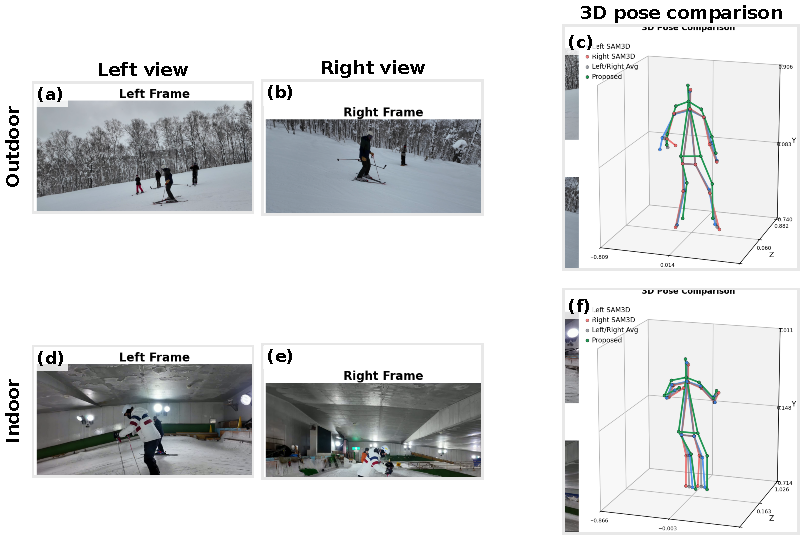
\includegraphics[width=0.98\textwidth]{figures/journal/realworld_qualitative.pdf}
\caption{Qualitative outputs on author-collected outdoor and indoor skiing videos. Panels (a), (b), (d), and (e) show the synchronized input views; panels (c) and (f) compare the two single-view predictions, canonical average, and CanonFuse3D output. These videos have no independent metric 3D annotations and are not used for training or quantitative evaluation. These examples were also included in the earlier conference manuscript.}
\label{fig:real_world_comparison}
\end{figure}

Figure~\ref{fig:real_world_comparison} illustrates deployment on the author-collected skiing videos, where left- and right-view poses are estimated independently and no camera calibration is used during inference. The proposed result remains more coherent than either single-view prediction or direct averaging, especially when the two views disagree around arms, knees, and feet. Because no independent 3D ground truth is available, this comparison is qualitative and is not included in any reported accuracy metric. The examples also show the main limitation: if both upstream predictions contain similar errors, the refinement can still inherit part of that error.

Qualitatively, the refined skeleton tends to preserve the more stable limb configuration while avoiding abrupt compromises caused by direct averaging. This is particularly visible in poses with strong torso rotation, occluded lower limbs, or large differences between left- and right-view predictions. For sports analysis, such behavior is useful because downstream measures such as joint-angle trajectories, limb extension timing, and motion smoothness are sensitive to frame-level outliers. At the same time, the examples should be read as a post-estimation refinement result rather than as full 3D reconstruction from images; the method improves the consistency of available pose streams but does not recover information that is absent from both inputs.

\FloatBarrier
\section{Discussion}
\DIFaddbegin \label{sec:discussion}
\DIFaddend 

The \DIFdelbegin \DIFdel{expanded main comparisons qualify the clean-input accuracy claim. A simple framewise MLP outperforms }\DIFdelend \DIFaddbegin \DIFadd{main comparison places }\DIFaddend CanonFuse3D \DIFdelbegin \DIFdel{in MPJPE }\DIFdelend \DIFaddbegin \DIFadd{between two groups of references. Among methods that receive only the two 3D pose streams, it outperforms every non-learned baseline }\DIFaddend on both datasets \DIFdelbegin \DIFdel{, and SmoothNet gives lower acceleration error}\DIFdelend \DIFaddbegin \DIFadd{in position, Procrustes-aligned, and acceleration error, and the margin over pose-space alignment alone shows that the learned gate and residual contribute beyond coordinate normalization. Against learned references the picture is metric-dependent: CanonFuse3D is more accurate than the temporal convolutional baseline on Unity, whereas that baseline reaches lower position error on the 30-sequence Ski-PTZ-Pose index, and SmoothNet attains the lowest acceleration error on both datasets while leaving the position error near canonical averaging. The calibrated group shows what additional information buys: plain triangulation of the estimated 2D joints is less accurate than the pose-only fusion, and only a learned correction on top of it surpasses CanonFuse3D. For field capture in which calibration is unavailable, the pose-only result is the relevant operating point}\DIFaddend . The \DIFdelbegin \DIFdel{present evidence therefore supports the measured operating behavior of this refinement design, not a general claim that cross-view attention or reliability gating is required to obtain the best clean-input result . The added baselines were evaluated on the clean fixed indices. The }\DIFdelend perturbation, transfer, and view-scaling studies \DIFdelbegin \DIFdel{retain their stated comparison methods, principally canonical averaging; they do not establish robustness superiority over the newly added MLP, TCN, SmoothNet, or calibrated pipelines.
}%DIFDELCMD < \label{sec:discussion}
%DIFDELCMD < %%%
\DIFdelend \DIFaddbegin \DIFadd{compare against canonical averaging, the non-learned reference that shares the model's inputs; they characterize the operating range of CanonFuse3D rather than rank fusion architectures under perturbation.
}\DIFaddend 

The combined evidence supports a narrower claim than generic calibration-free multi-view reconstruction. CanonFuse3D is effective as a pose-space refinement layer when its two inputs are approximately synchronized, share the training front end's error distribution, and contain complementary evidence. It requires no camera parameters and retains a large advantage across the tested Unity angle bins. Pairwise composition extends the frozen dual-view model to larger camera groups, but it does not learn a joint representation over more than two views. Under the evaluated serial implementation, the number of forwards grows from one pair at two views to three and six pairs at three and four views, increasing latency from 2.02~ms to 6.02 and 12.06~ms. Because two views capture the largest accuracy gain over a single view while additional views provide smaller improvements at approximately threefold and sixfold latency, the dual-view configuration is the main accuracy--cost operating point. This timing conclusion is implementation-specific: batching or parallelizing independent pairs could reduce wall-clock latency without changing the pair count. Likewise, tolerance to small time and clock perturbations does not establish robustness to unknown long delays, dropped frames, or independently varying frame rates.

The \DIFdelbegin \DIFdel{frozen }\DIFdelend front-end \DIFdelbegin \DIFdel{comparison identifies the main deployment limitation. MotionBERT preserves a modest positive gain, whereas VideoPose3D and PoseFormer do not. This result rules out an }\DIFdelend \DIFaddbegin \DIFadd{experiments delimit the generalization claim. The architecture is }\DIFaddend estimator-agnostic \DIFdelbegin \DIFdel{interpretation of the current checkpoint. The adaptation matrix therefore tests heads-only, full-model, and mixed-front-end updating while retaining native-SAM3D evaluation as a forgetting check}\DIFdelend \DIFaddbegin \DIFadd{and, after 20 epochs of adaptation on training and validation data, improves over canonical averaging on every tested front end, whether adapted to one target or to a mixture; a single mixed model serves all four. What does not transfer is a frozen checkpoint: the fusion weights are coupled to the error distribution of the estimator they were trained on, so deploying CanonFuse3D behind a new estimator should include a short adaptation step, and the adaptation trades native-front-end retention against target recovery}\DIFaddend . The alternative-front-end \DIFdelbegin \DIFdel{transfer and adaptation experiments still }\DIFdelend \DIFaddbegin \DIFadd{experiments }\DIFaddend use ground-truth Unity 2D tracks to isolate 3D lifting; comparisons that include image-detection noise for those estimators remain necessary.

The image-level study broadens the native-SAM3D evidence to include synthetic RGB occlusion and upstream detection failures. Gains in 15 of 18 conditions support a useful operating range, while the three random ratio-1.0 failures show that an unoccluded second view alone is insufficient to ensure an improvement over averaging. The masking study uses Unity projections to place artificial patches and one frozen SAM3D front end. It does not establish robustness to natural occluders, weather, motion blur, or image-level errors from alternative estimators. Those settings require separate evaluation, and the observed association between detection failures and fusion degradation does not identify a causal mechanism.

Motion blur can affect the refinement through a different error process. During an exposure, fast limb motion or camera motion spreads image evidence along a trajectory, which can reduce joint-localization reliability or cause the front end to miss the person. The resulting 3D errors may persist across adjacent frames, altering both velocity features and cross-view disagreement. A clearer second view may provide useful evidence, but similar blur-induced errors in both streams can leave the gate with little reliable information to select. Errors in the hip or neck landmarks used for the batch anchor can additionally perturb the coordinate transform. These are expected mechanisms, not measured blur effects in this study. Temporal refinement may suppress isolated jitter, but neither temporal smoothing nor the reported patch-occlusion results establish robustness to exposure-induced motion blur.

The reference regimes constrain interpretation. Unity provides an avatar skeleton in dataset coordinates that is transformed using the same batch-referenced rule; it is not a metric motion-capture measurement. Ski-PTZ-Pose is evaluated against a transformed fused reference derived from view-specific annotations; its result measures agreement with that constructed reference rather than independent physical 3D accuracy. Raw-space and transformed-space errors are therefore not interchangeable, no skeleton-scale normalization is performed, and none of these values should be relabeled as millimeters.

The body reference is shared within each evaluated batch, so changing its composition can change the representation. The results do not establish invariance to regrouping or single-sequence deployment. A sample-independent variant would require retraining and evaluation; the exact reference convention is documented in Supplementary Section~\ref{S-sec:implementation_record}.

The reliability gate is informative but not calibrated uncertainty. Its mean is explicitly shaped by balance and entropy regularization, so high gate-error correlation and preference accuracy do not establish probabilistic calibration. Because the frozen-checkpoint stress tests reuse one trained checkpoint, they do not quantify variation across independent training runs. Between-dataset uncertainty also remains unresolved. External sports datasets, metric 3D references, longer asynchronous sequences, and naturally occurring image degradation remain necessary directions.

\section{Conclusion}
\label{sec:conclusion}

CanonFuse3D shows that human-centric fusion can refine two independently estimated 3D pose streams without camera parameters. Pose alignment, cross-view temporal features, and gated residual correction \DIFdelbegin \DIFdel{improve agreement with the evaluated references over canonical averaging when the inputs provide complementary evidence}\DIFdelend \DIFaddbegin \DIFadd{reduce the position error relative to canonical averaging by 44.5\% on Unity and 48.6\% on Ski-PTZ-Pose and outperform every non-learned fusion baseline in position, Procrustes-aligned, and acceleration error, while a temporal convolutional baseline is competitive in position error and a temporal smoother trades position accuracy for temporal smoothness}\DIFaddend . The benefit \DIFdelbegin \DIFdel{is conditional: severe corruption and a changed upstream error distribution can reverse it, and simple learned baselines achieve lower clean-input position or acceleration errors. The }\DIFdelend \DIFaddbegin \DIFadd{persists across camera separations, small timing and sampling-rate errors, and structured pose or image occlusion, and it is reversed only by dense corruption of both inputs. The same architecture adapts to alternative upstream estimators with lightweight fine-tuning and extends to three and four cameras through pairwise composition, with two views remaining the most favorable accuracy--cost operating point. The }\DIFaddend findings support calibration-free post-estimation dual-view \DIFdelbegin \DIFdel{refinement as a useful component for difficult moving-subject capture }\DIFdelend \DIFaddbegin \DIFadd{fusion as a practical component for distant capture of rapidly moving subjects}\DIFaddend , while emphasizing \DIFdelbegin \DIFdel{the need to validate }\DIFdelend \DIFaddbegin \DIFadd{that a frozen fusion model should be validated, and if necessary adapted, for }\DIFaddend the chosen pose estimator and capture conditions.

\section*{Acknowledgments}
We thank the dataset providers and the open-source research community for making this work possible. This research, in part, used computational resources of Pegasus provided by the Multidisciplinary Cooperative Research Program in the Center for Computational Sciences, University of Tsukuba. This work used computational resources of Pegasus provided by University of Tsukuba through the HPCI System Research Project (Project ID: hp260146).

\section*{Declaration of competing interest}
\textbf{Author confirmation required before submission.} The authors must approve the final declaration wording.

\section*{CRediT authorship contribution statement}
\textbf{Author confirmation required before submission.} Contributions must be approved by all seven authors.

\section*{Data and code availability}
Ski-PTZ-Pose is available from the dataset provider~\cite{ski_poseptz_dataset}. The release status and repository URL for the Unity data, trained checkpoint, evaluation manifests, and evaluation scripts must be confirmed by the authors before submission. The author-collected indoor and outdoor videos are used only for qualitative illustration; their sharing conditions must also be confirmed before submission. The local reproducibility package records exact checkpoint and estimator hashes.

\section*{Ethics and generative-AI disclosure}
The quantitative study uses a synthetic dataset and a previously released research dataset. The author-collected indoor and outdoor videos are used solely for qualitative illustration and do not contribute training samples or quantitative measurements. The authors must confirm and report any applicable institutional-review and participant-consent requirements for these recordings before submission. Journal-required disclosure of generative-AI assistance must also be reviewed and approved by the authors before submission.

\setlength{\bibsep}{4pt}
\bibliographystyle{elsarticle-num}
\bibliography{references}

\end{document}
